\chapter{Cmake}

\section{Overview}

Cmake is super old. It has more than 300 functions.
Yet, modern cmake only need 50. 250 should not be used, increasing difficulty.
Older tutorials are confusing.

Modern cmake emphases readability, older functions complexify.

\section{Compilers}

If your program has 3 .cpp files, the compiler would generate 3 object files. 
After all object files were compiled, the linker starts. 

\begin{center}
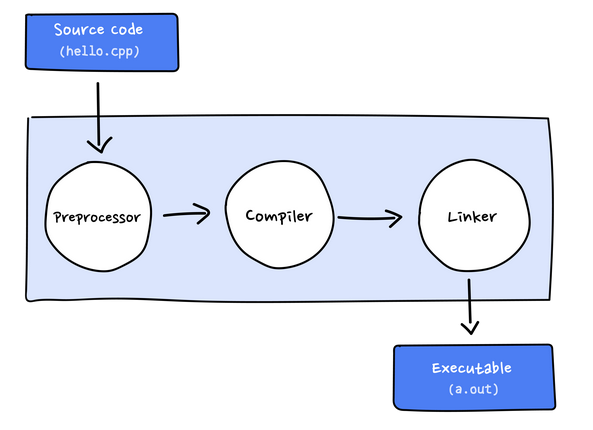
\includegraphics[width=3.5in]{compile.png}
\end{center}

\begin{center}
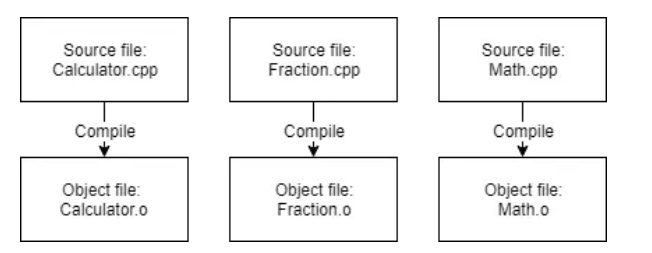
\includegraphics[width=3.5in]{compiling.png}
\end{center}

\begin{verbatim}
MVSC        // Microsoft Compiler
GCC         // Gnu C Compiler
LLVM Clang  // LLVM Compiler
\end{verbatim}

\subsection{Compile}
\begin{verbatim}
g++ hello.cpp -o hello

Compiling translates C++ programs into machine code.
It is stored on disk as a file with the .o extension (hello.o). 
\end{verbatim}

A linker then links the object code with standard library routines
that the program may use and creates an executable image which is also saved on disk,

usually as a file with the file name without any extension (e.g. hello).

\section{Linkers}

\begin{verbatim}
    It combined all object files in one executable.
    the linker links library files. 
    resolves cross-file dependencies.  
\end{verbatim}

\begin{center}
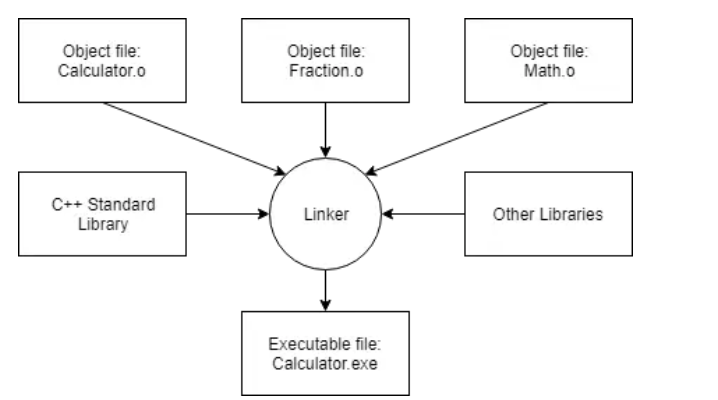
\includegraphics[width=4in]{linker.png}
\end{center}

\subsection{Link Header Files}

\begin{verbatim}
-- main.cpp --
#include "my_function.hpp"

$ g++ main.cpp my_function.cpp -o program

-- fun.hpp / fun.h --
double average(double num1, double num2);

-- fun.cpp --
double average(double num1, double num2) {
  return (num1 + num2) / 2;
}
\end{verbatim}

\subsection{Standard Library Headers}

\begin{verbatim}
Some standard library headers are included by others. 

<cstdlib> is included by <iostream>, since it relies on its functionalities,
such as the declaration of the system() function. 
\end{verbatim}

\section{Command Line Linking and Compiling}

\begin{verbatim}
g++ main.cpp my_functions.cpp // link both files
\end{verbatim}

\subsection{Source Code Files Suffix}

\begin{verbatim}
    .cpp (ex: hello.cpp) or
    .h (ex: std_lib_facilities.h).
\end{verbatim}


\section{Compiler Extensions (compiler-specific behavior)}


\textbf{This should not be in cmake, but in engineering}


Many compilers change the language through extentions. Non compliant c++ code is possible with them.
Extension are overpermissive and enabled by default.


Programs using non-standard extensions generally will not compile on other compilers 
(lacking same extensions support). If they do, they may not run correctly.

\begin{verbatim}
GCC
         -pedantic-errors // Disable extensions
\end{verbatim}

\section{Max Warnings}

\begin{verbatim}
GCC 
    -Wall -Weffc++ -Wextra -Wsign-conversion
    -Werror

Turner does it with cmake?
\end{verbatim}

\section{Standard Set-Up}

\begin{verbatim}
GCC pre-8
          -std=c++11 // set c++ standard
          -std=c++14
          -std=c++17
          -std=c++20 
GCC 8 or 9
          -std=c++2a for C++20 support

g++ -std=c++17 myfile.cpp -o output // cmd line
\end{verbatim}

\section{Precompiled Headers (PCH)}

Speed compilation in larger projects. A PCH file make subsequent compilations faster.




\section{Debugg and Error Type}

\subsection{Compile Time Errors}

\subsection{Synthax Errors}

\subsection{Type errors}

Forgetting to declare a variable

Storing a value in a different type. 

\subsection{Link-Time Errors}

link-time errors are based on unfindable needed function or library.

When the linker tries to combine object files into an executable.

\subsection{Run-Time Errors}

Errors which happen during program execution (run-time) after successful compilation.

Division by zero

Open an non-existing file

\subsection{Logical Errors}

Flawed programming's logical thinking. 

No errors, but output is wrong. 

\section{Project Structure}

\begin{center}
    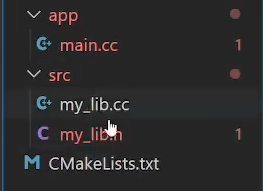
\includegraphics[width=2in]{cpp_tree1.png}
\end{center}

\subsection{App Directory}

Define everything important for the executable target, including its own CMakeLists.txt.

\subsection{Source Directory - src}

Define everything important for our library. When you have multiple libraries, create multiple directories in
src. As a naming convention, the subdirectory should have the same name as the library.

\begin{center}
    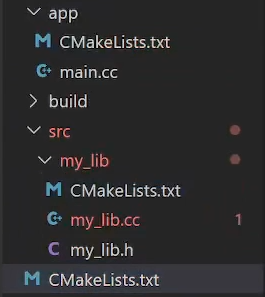
\includegraphics[width=2in]{cpp_tree3.png}
\end{center}

Don't forget to add a CMakeList in the src directory.


\begin{center}
    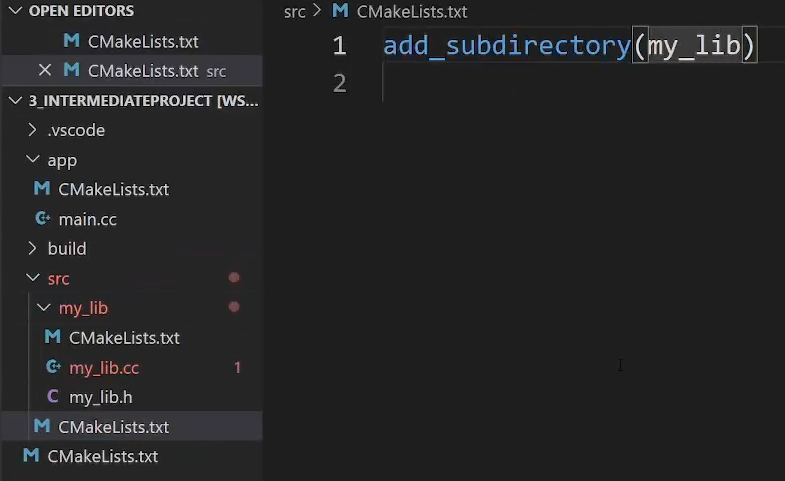
\includegraphics[width=4in]{cpp_tree4.png}
\end{center}

\subsection{CMake Default Paths}

Cmake has built-in paths to use. We use many in these notes.

\begin{verbatim}
# CMAKE_SOURCE_DIR is always the directory of the
# root CMakeLists.txt file
# our root directory

# CMAKE_BINARY_DIR is always our build directory
\end{verbatim}

\section{Variables}

You can create variables for your executable or your libraries in the root CMakeLists.txt. Variables
will be usable in all add\_subdirectory chain at the end of the same document.

\begin{verbatim}
# set a variable for the library you want to use
# common synthax is capital letters.

# we reference Library in other CMakeLists files
# we change the Library name for LIBA

set(LIBA Library)

# where we used Library, write ${LIBA}


# we have used Hello for our executable name so far.
# we can change it as well.
set(HE Hello)

# where we used Hello, write ${HE}

add_subdirectory(src)
add_subdirectory(app)
\end{verbatim}


\subsection{Standard for cpp}

Specify your C++ standard. Essential to overwrite the compiler defaults
(with huge variability between compiler versions!).
In your root CMakeLists.txt file define a variable and sets the standard to 17.

\begin{verbatim}
set(CMAKE_CXX_STANDARD 17)
set(CMAKE_C_STANDARD 98)
\end{verbatim}

\subsection{Standard Required}

Indicate that the compiler 100 pourcent implemented the language's standard.

\begin{verbatim}
set(CMAKE_CXX_STANDARD 17)
set(CMAKE_CXX_STANDARD_REQUIRED ON)
\end{verbatim}

\subsection{Compiler Extensions}

\begin{verbatim}
set(CMAKE_CXX_STANDARD 17)
set(CMAKE_CXX_STANDARD_REQUIRED ON)
set(CMAKE_CXX_EXTENSIONS OFF)
\end{verbatim}

\subsection{Conditional - If Statement}

\begin{verbatim}
option(COMPILE_EXECUTABLE "Whether to compile the executable" OFF)

add_subdirectory(src)

if (COMPILE_EXECUTABLE)
    add_subdirectory(app)
else()
    message("Without executable compiling")
endif()
\end{verbatim}


\section{Makefile Shell Scripting}

Make is Cmake's ancestor. You can automate folder creation and files,
like any shell script.
\textbf{Make do not support spaces, use tabs}.

\begin{verbatim}
prepare:
    rm -rf build
    mkdir build
    cd build

$ make prepare # execute 
\end{verbatim}

\section{Command Line Options}

\subsection{Custom Command Line Options}

You can set an option,
the second argument is a simple comment for the reader (with no impact).

\begin{verbatim}
option(COMPILE_EXECUTABLE "Whether to compile the executable" OFF)

add_subdirectory(src)

if (COMPILE_EXECUTABLE)
    add_subdirectory(app)
endif()

# to call the option from the command line

#$ cmake .. -DCOMPILE_EXECUTABLE=ON
#$ cmake .. -DCOMPILE_EXECUTABLE=OFF
\end{verbatim}


\subsection{Generating a Project}

\begin{verbatim}
cmake [<options>] -S <path-to-source> -B <path-to-build>
\end{verbatim}

Assuming that a CMakeLists.txt is in the root directory, you can generate a project like the following.

\begin{verbatim}
mkdir build
cd build
cmake -S .. -B . # Option 1
cmake .. # Option 2

Assuming that you have already built the CMake project, you can update the generated project.

cd build
cmake .
\end{verbatim}

\subsection{Generator for GCC and Clang}

\begin{verbatim}
cd build
cmake -S .. -B . -G "Unix Makefiles" # Option 1
cmake .. -G "Unix Makefiles" # Option 2
\end{verbatim}

\subsection{Generator for MSVC}

\begin{verbatim}
cd build
cmake -S .. -B . -G "Visual Studio 16 2019" # Option 1
cmake .. -G "Visual Studio 16 2019" # Option 2
\end{verbatim}

\section{Builds Type}

Per default, the standard type is in most cases the debug type.
If you want to generate the project, for example, in release mode you have to set the build type.

\begin{verbatim}
cd build
cmake -DCMAKE_BUILD_TYPE=Release ..
\end{verbatim}

\subsection{Passing Options}

If you have set some options in the CMakeLists, you can pass values in the command line.

\begin{verbatim}
cd build
cmake -DMY_OPTION=[ON|OFF] ..
\end{verbatim}

\subsection{Specify the Build Target (Option 1)}

The standard build command would build all created targets within the CMakeLists.
If you want to build a specific target, you can do so.

\begin{verbatim}
cd build
cmake --build . --target ExternalLibraries_Executable
\end{verbatim}

The target ExternalLibraries\_Executable is just an example of a possible target name.
Note: All dependent targets will be built beforehand.

\subsection{Specify the Build Target (Option 2)}

Besides setting the target within the cmake build command, you could also run the previously generated Makefile (from the generating step).
If you want to build the ExternalLibraries\_Executable, you could do the following.

\begin{verbatim}
cd build
make ExternalLibraries_Executable
\end{verbatim}

\section{Run the Executable}

After generating the project and building a specific target, run the executable.
The main.cpp file of the executable is in the app dir. 

\begin{verbatim}
cd root/build/app
./program_executable
\end{verbatim}

\section{Configuration - Precompiling Information}

Create a configuration directory. With a config.hpp.in file.

\begin{center}
    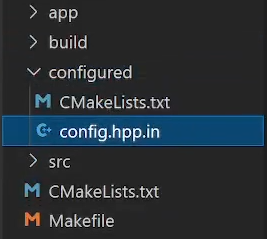
\includegraphics[width=2in]{conf.png}
\end{center}

In the CMakeLists.txt of this new configured directory.

\begin{verbatim}
configure_file(
    "config.hpp.in"
    # "${CMAKE_BINARY_DIR}" this is our build directory
                          # it is one of prebuilt directories in CMAKE
                          # thus, we reference it with CMAKE_BINARY_DIR
                          # we create an output for a config file, 
                          # in our build directory.

    # "${PROJECT_SOURCE_DIR}" # stores absolute path to project's root directory

    "${CMAKE_BINARY_DIR}/configured_files/include/config.hpp" ESCAPE_QUOTES)
\end{verbatim}

\subsection{Project Version Number}

In config.hpp.in

\begin{verbatim}
# @ cmake looks for and remplaces text between @@ this text @

#include <cstdint>
#include <string_view> 
static constexpr std::string_view project_name = "@PROJECT_NAME@";
static constexpr std::string_view project_version = "@PROJECT_VERSION@";
\end{verbatim}

\subsection{Sementic Versioning}

In version names: 1.0.0 . This is the first Major version (1). Incrementing the major version means
that the previous and the new codebase are not compatible at all. 2.0.0 have breaking changes with the 1.0.0 version.

The minor version 1.6.0, number 6 here, indicate that new features are available. Yet, nothing breaks between minor versions.

The patches are the last number, the last small fixes.

\begin{verbatim}
static constexpr std::int32_t project_version_major{@PROJECT_VERSION_MAJOR@};
static constexpr std::int32_t project_version_minor{@PROJECT_VERSION_MINOR@};
static constexpr std::int32_t project_version_patch{@PROJECT_VERSION_PATCH@};

#### Resulting file looks like.

#pragma once

#include <cstdint>
#include <string_view>

static constexpr std::string_view project_name = "CppProjectTemplate";
static constexpr std::string_view project_version = "1.0.0";

static constexpr std::int32_t project_version_major{1};
static constexpr std::int32_t project_version_minor{0};
static constexpr std::int32_t project_version_patch{0};
\end{verbatim}


\section{Sources and Headers}

When you have many libraries and many headers, create a variable for all of your headers.
Then, reference this variable to include everything.
List all of your source files in my\_lib directory.

\begin{verbatim}
set(LIBRARY_SOURCES
     "my_lib.cpp"
     "my_lib2.cpp"
     ) # quotes are not mandatory, just preference.
set(LIBRARY_HEADERS
     "my_lib.h")

add_library(${LIBRARY_NAME} STATIC
    "./"
    "${CMAKE_BINARY_DIR}/configured_files/include")
\end{verbatim}

\subsection{Executables}

You can do the same thing if you generate many executables, I think. This would be in your app directory.

\begin{verbatim}
set(EXE_SOURCES
    "main.cpp")

add_executable(${EXECUTABLE_NAME} ${EXE_SOURCES})
target_link_libraries(${EXECUTABLE_NAME} PUBLIC ${LIBRARY_NAME})
\end{verbatim}


\section{External Libraries}


\subsection{Git Submodule - nlohman json}

Create an external directory. Our project looks like this:

\begin{center}
    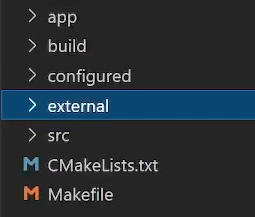
\includegraphics[width=2in]{external.png}
\end{center}

\begin{verbatim}
// make sure that your root folder is a git repo, git init

git submodule add https://github.com/nlogmann/json external/json

// it creates the json directory, when cloning the module in it.
\end{verbatim}

\subsection{Custom Cmake Functions}

In a cpp project, when you create your own cmake functions, they are stored in a Cmake directory. We just cloned a 
git repo in our external directory.

\begin{center}
    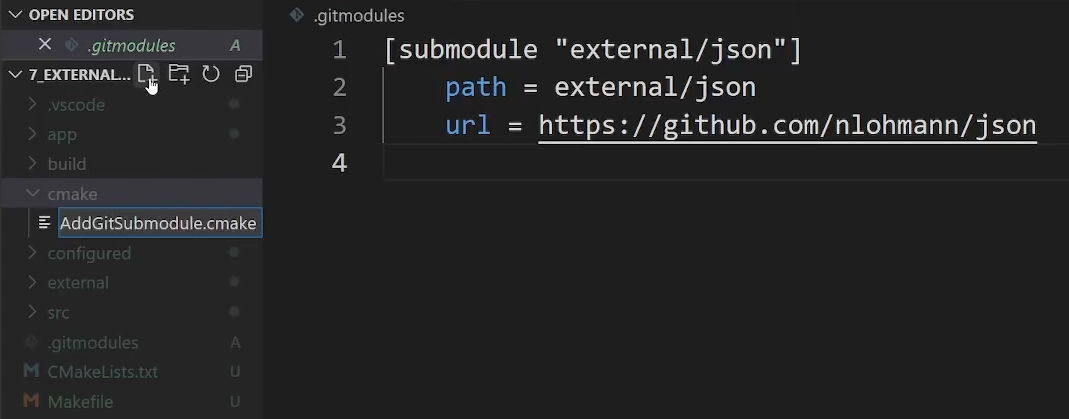
\includegraphics[width=4in]{add.png}
\end{center}

Now we create a AddGitSubmodule.cmake file. Inside, we define our function.

\begin{verbatim}
function(add_git_submodule dir)    # our function takes one argument called dir
                                   # this dir, is where the submodule is located
                                   # making the add_ action possible.

        find_package(Git REQUIRED) # Git must be on your computer, or it
                                   # Error's out.

        if (NOT EXISTS ${dir}/CMakeLists.txt)
            execute_process (COMMAND ${GIT_EXECUTABLE}}
            submodule update --init --recursive -- ${dir}

                                   # recursive is essential here
                                   # If someone clones your project, 
                                   # It automatically clones this submodules,
                                   # It clones auto repos, inside your repo.
                                                            
            WORKING_DIRECTORY ${PROJECT_SOURCE_DIR}) 
                                   # cmake saves some variable
                                   # including the source dir
                                   # of our project.
        endif()
        
        if (EXISTS ${dir}/CMakeLists.txt)
            message("Adding ${dir}/CMakeLists.txt")
            add_subdirectory(${dir})
        else
            message("Could not add ${dir}/CMakeLists.txt")
        endif()
endfunction(add_git_submodule)
\end{verbatim}

\subsection{Log example}

Here we are using an external library called log, with only two files, log.c and log.h . We have the library in our 
external directory. Plus, we have a CMakeLists.txt at the root of the external folder, taking care of the log library. 

\begin{center}
    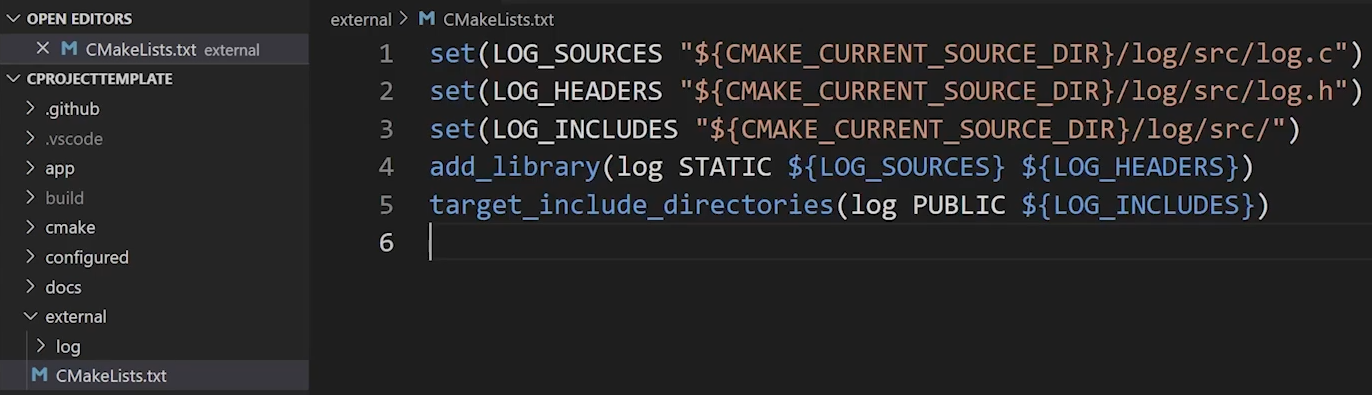
\includegraphics[width=6in]{loge.png}
\end{center}

\subsection{Call Your Own Functions}

In the source CMakeFiles.txt, knowing that we have a new git submodule.

\begin{verbatim}
set(CMAKE_MODULE_PATH "${PROJECT_SOURCE_DIR}/cmake")
include(AddGitSubmodule) # includes indicates thats it a cmake module file.
                         # it will look where cmake modules are defined
                         # in our cmake dir


add_git_submodule(external/json) # this calls our custom function.

# In our app, we add this as well

set(EXE_SOURCES
    "main.cpp")

add_executable(${EXECUTABLE_NAME} ${EXE_SOURCES})
target_link_libraries(${EXECUTABLE_NAME} PUBLIC
    ${LIBRARY_NAME}
    nlohmann_json) # this links the submodule with the executable

# In main.cpp, we add 

#include <nlohman/json.hpp>
\end{verbatim}


\subsection{Fetch Content (fmt, spdlog, cxxopts, catch2)}

We have the gitmodule example, but modern CMake has a great fetching feature. Our root CMakelLists.txt will look like this, 

\begin{verbatim}
...

set(CMAKE_MODULE_PATH "${PROJECT_SOURCE_DIR}/cmake/")
include(AddGitSubmodule)


include(FetchContent)  # built-in library or file
                       # including it gives access to features

FetchContent_Declare() # Declare which github repository we would like to use
FetchContent_MakeAvailable() # will load this library in our cmake project.


                       # I want to use github.com/nlohmann/json
                       # any Gitlab is also possible
                       # I can do:
FetchContent_Declare(
    nlohmann_json      # since this repo is a cmake project,
                       # look at the project's root CMakeLists.txt file
                       # you will the name of the project, to enter here 
                       # see next image

    GIT_REPOSITORY https://github.com/nlohmann/json
    GIT_TAG v3.11.2    # the version I want to use
    GIT_SHALLOW TRUE)  # The function won't clone the repo recursively

                       # With this function, the git repository will be cloned in  
                       # our cloned repository.
                       # And it needs to be a cmake project.

                       # if it is not a cmake project, use the AddGitSubmodule method shown.
FetchContent_MakeAvailable(nlohmann_json) # will load this library in our cmake project.
\end{verbatim}

\begin{center}
    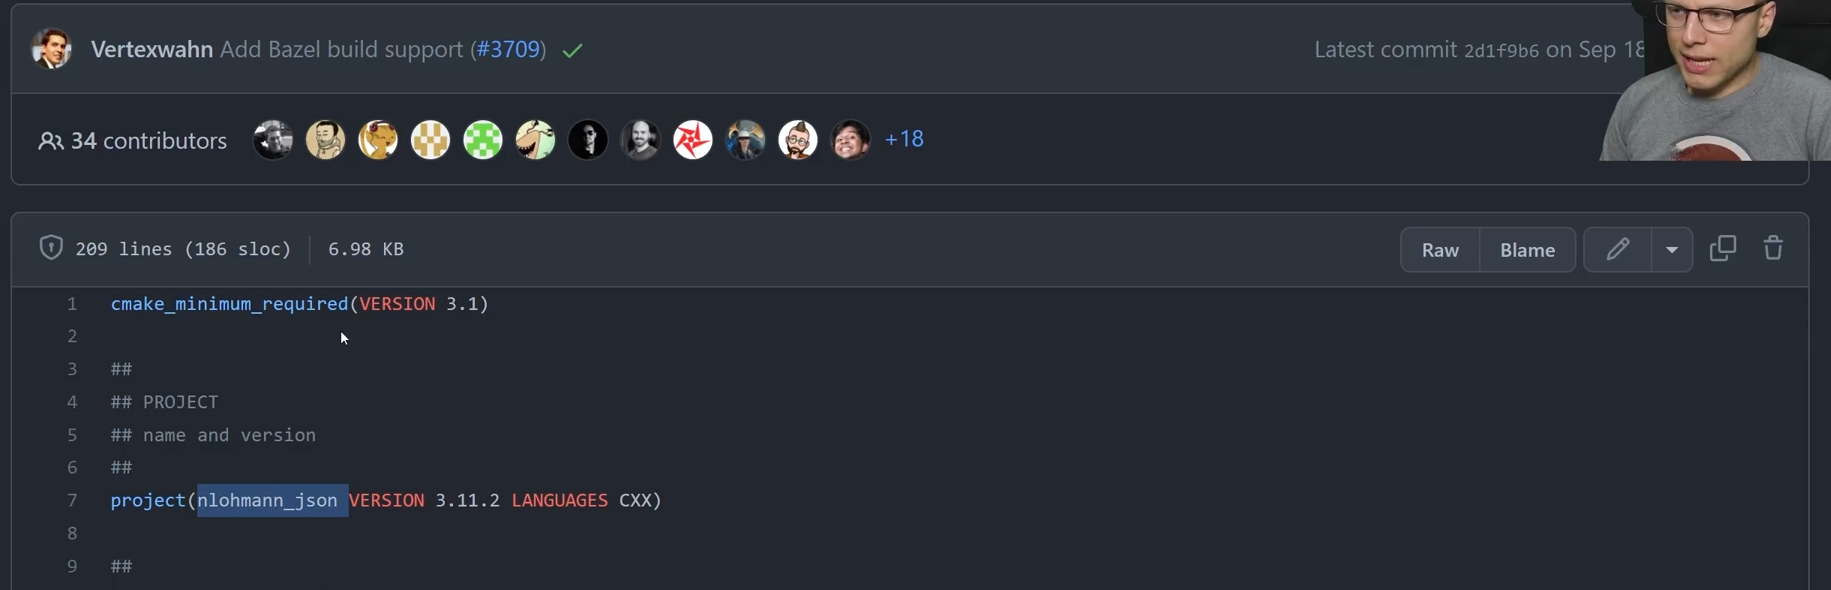
\includegraphics[width=5in]{json_n.png}
\end{center}


\subsubsection{FMT}

The best library to easily format strings in cpp.

\begin{verbatim}
FetchContent_Declare(
    fmt
    GIT_REPOSITORY https://github.com/fmtib/fmt
    GIT_TAG 9.1.0
    GIT_SHALLOW TRUE)
FetchContent_MakeAvailable(fmt)
\end{verbatim}

\subsubsection{spdlog}

The best fast logging library for cpp.

\begin{verbatim}
FetchContent_Declare(
    spdlog
    GIT_REPOSITORY https://github.com/gabime/spdlog
    GIT_TAG v1.11.0
    GIT_SHALLOW TRUE)
FetchContent_MakeAvailable(spdlog)
\end{verbatim}

\subsubsection{Cxxopts}

The best library to work with command line arguments in cpp. From the received arguments, to any other type.
The equivalent of the argument parser in python.

\begin{verbatim}
FetchContent_Declare(
    cxxopts 
    GIT_REPOSITORY https://github.com/jaroo2783/cxxopts
    GIT_TAG v3.0.0
    GIT_SHALLOW TRUE)
FetchContent_MakeAvailable(cxxopts)
\end{verbatim}

\subsubsection{Catch2}

The best Unit Testing library, seen further below.

\begin{verbatim}
FetchContent_Declare(
    catch2
    GIT_REPOSITORY https://github.com/catchorg/Catch2
    GIT_TAG v2.13.9  # teacher recommended this version, not the latest.
    GIT_SHALLOW TRUE)
FetchContent_MakeAvailable(catch2)
\end{verbatim}


\subsubsection{Include All Libraries in root CMakeListstxt}

Refer to Final project Template seen in the course. Modifying the CMakeLists.txt in our my-lib directory.

\begin{center}
    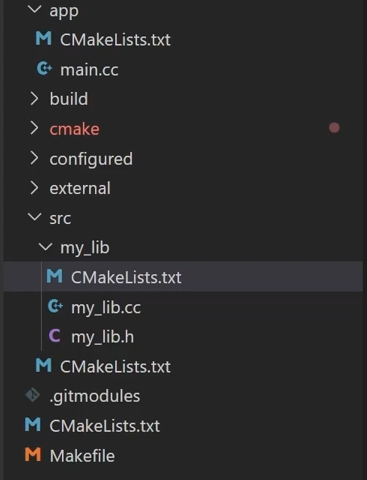
\includegraphics[width=2in]{final_p.png}
\end{center}

\begin{verbatim}
set(LIBRARY_SOURCES
    "my_lib.cpp")
set(LIBRARY_HEADERS
    "my_lib.h")
set(LIBRARY_INCLUDES
    "./"
    "${CMAKE_BINARY_DIR}/configured_files/include")

add_library(${LIBA} STATIC
    ${LIBRARY_SOURCES}
    ${LIBRARY_HEADERS})
target_include_directories(${LIBA} PUBLIC
    ${LIBRARY_INCLUDES})
target_link_libraries(${LIBA} PUBLIC
                                        # Naming convention is project_name::library_name
                                        # see next image, to find library_name in CMake project
                                        # on github
    
    nlohmann_json::nlohmann_json
    fmt::fmt
    spdlog::spdlog
    catch2::catch2
    cxxopts::cxxopts                    # not always the same

    )
\end{verbatim}

When this is set-up, and we reconfigure our cmake project, the repository will be cloned in a \_deps directory.
This includes a build, subbuild and src directory for all dependencies. Don't worry about it for now.

\begin{center}
    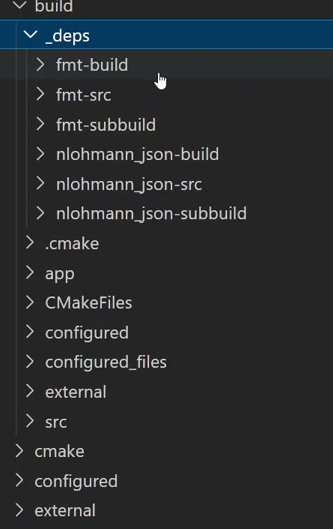
\includegraphics[width=2in]{deps.png}
\end{center}


\subsection{Include All Libraries in App Main.cpp}

It is tricky to include the libraries files in main. Some have directories, some do not.

\begin{verbatim}
#include <iostream>

#include <cxxopts.hpp>
#include <nlohman/json.hpp>
#include <fmt/format.h>
#include <spdlog/spdlog.h>
#include <catch2>

#include "my_lib.h"
#include "config.hpp"

int main() {
    ...
    std::cout << "CXXOPTS: # chose any included lib, to prove you have access to their info

    << CXXOPTS__VERSION_MAJOR << "."
    << CXXOPTS__VERSION_MINOR << "."
    << CXXOPTS__VERSION_PATCH << "." # if you have access to these variable, 
                                     # you have successfully imported and configure the lib
                                     # for you project.

    ...

}
\end{verbatim}


\subsection{Git Submodules vs Fetch Content}

If the repo is not a CMakeProject, you should use Git Submodules. Valid for GitHub and GitLab. In this case, 
define its own library target, I think. Not explained in detail.

If it is a CMake project on GitHub or Gitlab, use FetchContent. It is easier to use, you don't need to mess with header
libraries or anything. We can simply use the makeAvailable and prepare function.

The instructor highly recommends FetchContent!


\chapter{CMake Package Managers}

\section{CPM - Cmake Package Manager}

There are a few ways to include external libraries in you project. Git submodules, fetch content and packages managers such as
Cmake Package Manager.

On CPM's github page, click Releases. Pick the latest release, download the CPM.cmake file and copy it to your project's
cmake directory.

\begin{center}
    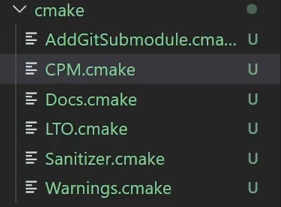
\includegraphics[width=2in]{cpm1.png}
\end{center}


\subsection{CPM Configuration in Root CMakeLists.txt}

Add an option in your root CMakeLists.txt.
Since the course's project has two different ways to import external libraries,
we will have an option for cpm and for fetch content.
We shouldn't use multiple tools at the same time. Thus, code
an if statement to use one or the other fetching method.

\textbf{Every external libraries used under CPM need to be github CMake projects, which 95 pourcent are.
It shouldn't be a problem}.


\textbf{Under the hood, CPM uses fetchcontent}. Therefore, the linking,
in the src/my\_lib/CMakeLists.txt file target\_link\_libraries function, 
can keep the fetchcontent synthax of nlohman\_json::nlohman\_json.


\begin{verbatim}
option(USE_CPM "Whether to use CPM" ON)

if(USE_CPM)
    message(STATUS "Using Cmake Package Manager")
    include(CPM)            # this includes the cpm.cmake file
    


                # "gh" cpm will look at github
                # "gh:nholmann" username
                # "gh:nholmann/json" repository name
                # "gh:nholmann/json#v3.11.2" version number 

    cpmaddpackage("gh:nholman/json#v3.11.2")    # This is CPM's defined function
    cpmaddpackage("gh:fmtlib/fmt#9.1.0")
    cpmaddpackage("gh:gabime/spdlog#v1.11.0")
    cpmaddpackage("gh:jarro2783/cxxopts#v3.1.1")
    cpmaddpackage("gh:cathorg/Catch2#v2.13.9")

else()
    message(STATUS "Using FetchContent")

    FetchContent_Declare(
        nlohmann_json      
        GIT_REPOSITORY https://github.com/nlohmann/json
        GIT_TAG v3.11.2    
        GIT_SHALLOW TRUE)  
    FetchContent_MakeAvailable(nlohmann_json) # will load this library in our cmake project.

    FetchContent_Declare(
        fmt
        GIT_REPOSITORY ...

endif()
\end{verbatim}

\section{Conan}

A package manager for cmake projects, alternatives to CPM and fetchcontent. CPM and fetchcontent localy
clones github repositories in your build directory. Then they compile the library locally, on your machine. 


Conan has a different approach. In an online database, pre-compiled repositories are available.
Conan downloads these. It depends on the compiler, but it generally saves compilation time.
No need to compile locally.

Conan binaries are compiled as release builds, not as debug builds.

A drawback for Conan is the binary updates. There are many configuration possible, and many updates
to keep track of. Therefore, many popular libraries won't have a compiled version for our machine's
configuration. Too many possibilities, Conan can't keep up with updates.

\subsection{Conan Installation}

\begin{verbatim}
Official installation guide is [here](https://docs.conan.io/2/).

The conan database is [here](https://conan.io/center/).

1. Install Python (3.7+)
2. Type ``pip install --user -U conan`` into the terminal
   1. Unix: Append conan to the PATH by: ``source ~/.profile``
3. Run: $ conan

4. $ conan profile detect --force
5. $ conan profile path default
\end{verbatim}


\subsection{Conan Configuration in Root CMakeLists.txt}

There is a pattern here, when you want to use something new in your cmake project,
set an option in the CMakeLists.txt file first.

Since the course shared examples for GitSubmodules, FetchContent, CPM and Conan,
we have a large if statement in our root CMakeLists.txt. In a regular project, 
select the tool you want, you wouldn't need the if.

\begin{verbatim}
option(USE_CONAN "Whether to use CPM" ON)

if(USE_CPM)
    ...
elseif(USE_CONAN)
    message(STATUS "Using Conan")
    include(${CMAKE_BINARY_DIR}/conan_toolchain.cmake  
                                # This is generated by a conan command
                                # in the conanfile.py (generate)
                                # including it in advance here.
    find_package(nlohmann_json REQUIRED)
    find_package(fmtlib REQUIRED)
    find_package(spdlog REQUIRED)
    find_package(cxxopts REQUIRED)
    find_package(Catch2 REQUIRED)

else()
    FetchContent_Declare(
        ...
\end{verbatim}

\subsection{Conanfile.py}

To configure conan, create a conanfile.py in your root directory.

\begin{center}
    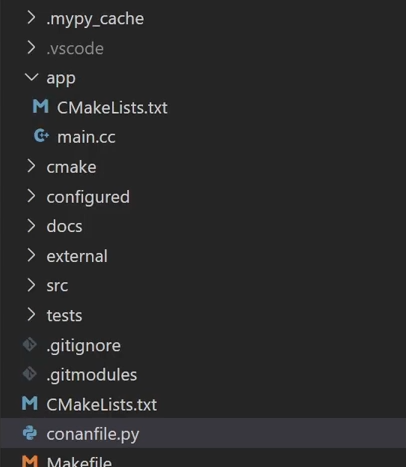
\includegraphics[width=2in]{conanfile.png}
\end{center}

\begin{verbatim}
from conan import ConanFile
from conan.tools.cmake import CMakeToolchain

class CompressorRecipe(ConanFile):
    settings = "os", "compiler", "build_type", "arch"
    generators = "CMakeDeps"

    def requirements(self):
        self.requires("nlohman_json/3.11.2")    # look at conan's database
                                                # to see which pre-compiled
                                                # versions are available
        self.requires("fmt/9.1.0")
        self.requires("spdlog/1.11.0")
        self.requires("catch2/2.13.9")
        self.requires("cxxopts/3.1.1")

    def generate(self):                         # this function generates the
                                                # conan_toolchain.cmake file
        tc = CMakeToolchain(self)
        tc.user_presets_path = False
        tc.generate()
\end{verbatim}

\subsection{Conan Debug Build}

Conan has release binaries by default, you have to tweak settings for you debug build.
To automatize conan's debug management, the instructor changed its makefile script.


\begin{verbatim}
conan_d:    # for conan debug
    rm -rf build
    mkdir build
    cd build && conan install .. -s build_type=Debug =s compiler.cppstd=17 --output-folder=. --build missing
                                -s               # for settings change
                                -- build missing 
                                                 # build binaries where no compiled version are available

conan_r:    # for conan release
    rm -rf build
    mkdir build
    cd build && conan install .. -s build_type=Release -s compiler.cppstd=17 --output-folder=. --build missing



### With this, run

$make conan_d
$make conan_r
\end{verbatim}  


\subsection{Conan Generated File}

Conan generates many files in your build directory, based on our configurations. Yet, no need to worry about them, conan
will deal with them.


\begin{center}
    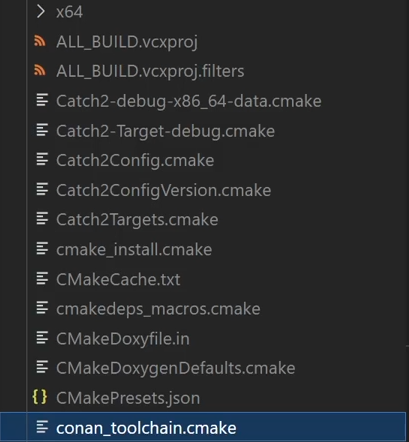
\includegraphics[width=2in]{conan2.png}
\end{center}

\section{VCPKG}

A C/C++ package manager for Microsoft. 
To use it, clone the VCPKG repository in your project's external library directory.

\begin{verbatim}
VCPKG database for available packages.

vcpkg.io/en/packages.html

Better is 

vcpkg.link 
\end{verbatim}

\subsection{VCPKG Installation}

Move to you project's external directory and clone the repo. Then, execute the .sh script.
 
\begin{verbatim}
Official Link: <https://vcpkg.io/en/index.html>

cd external
git clone https://github.com/Microsoft/vcpkg.git

.\vcpkg\bootstrap-vcpkg.bat  # windows
./vcpkg/bootstrap-vcpkg.sh   # Unix

cd vcpkg 
vcpkg --help 
\end{verbatim}


\subsection{VCPKG.json file in project root}

List dependencies of your cmake project in a JSON file. VCPKG's synthax is very tricky, plus its 
requirements are complicated for no reason.

It automatically downloads the latest versions of all libraries. Thus, if we want one particular
version, we need this overrides keyword.

\begin{verbatim}
{
    "name": "cpptemplateproject",
    "version-string": "1.0.0",
    "dependencies": [
        {
            "name": "cxxopts",
            "version>=": "3.1.1"
        },
        {
            "name": "fmt",
            "version>=": "9.1.0"
        },
        {
            "name": "nlohmann-json",
            "version>=": "3.11.2"
        },
        {
            "name": "spdlog",
            "version>=": "1.11.0"
        },
        {
            "name": "catch2",
            "version>=": "2.13.9"
        }
    ],
    "overrides": [
        {
            "name": "catch2",
            "version": "2.13.9"
        }
    ],
    "builtin-baseline": "40619a55c3e76dc4005c8d1b7395071471bb8b96"

    # this baseline is the hexadecimal value
    # of a certain VCPKG git commit

    # this is ridiculously complicated,
    # in this examples here, we git logged the external/vcpkg directory of our project.
}
\end{verbatim}


\begin{center}
    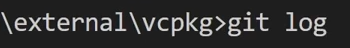
\includegraphics[width=2in]{ridiculous.png}
\end{center}


After configuration, libraries are downloaded and compiled on your system.


\begin{center}
    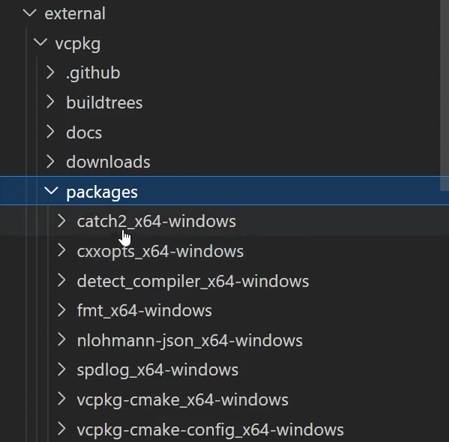
\includegraphics[width=2in]{vcpkg2.png}
\end{center}


\subsection{VCPKG configuration in root CMakeLists.txt}

Include vcpkg.cmake file in our project.

\begin{verbatim}
option(USE_CONAN "Whether to use CPM" ON)

if(USE_CPM)
    ...
elseif(USE_CONAN)
    message(STATUS "Using Conan")
    include(${CMAKE_BINARY_DIR}/conan_toolchain.cmake  
                                # This is generated by a conan command
elseif(USE_VCPKG)
    message(STATUD "Using VCPKG")

    include(${CMAKE_SOURCE_DIR}/external/vcpkg/scripts/buildsystems/vcpkg.cmake)
    find_package(nlohmann_json REQUIRED)
    find_package(fmt REQUIRED)
    find_package(..  REQUIRED)

else()
    FetchContent_Declare(
        ...
\end{verbatim}

\section{Package Managers Summary}

There are many ways to add and include libraries to our cmake project: Git Submodules, FetchContent,
Cmake Package Manager (CPM), Conan and VCPKG.

Use Git Submodules if you github repo you want to use is not a cmake project. It is a rare case, but it is
the best solution. Do not use this approach if they are cmake projects.


\textbf{CPM is the instructors' recommendation} for all gitlab and github cmake projects. However, it is important to understand the FetchContent functions of 
CMake. CPM uses these same fetch content methods under the hood.


VCPKG is hard to configure and version download complications. Not recommended.

Conan's pre-built binaries are a great idea, but they do not update these binaries often enough. 
However, if you have huge libraries that take 30 minutes to compile. Conan is the way to go.

\chapter{CMake Tooling}

\section{Dependency Graphs}

In a makefile, or any script, use the command --graphviz. Dependency and prepare are the flag needed to run the command.

\begin{verbatim}
dependency:
    cd build && cmake .. --graphviz=grap.dot && dot -Tpng graph.dot -o grapImage.png
                        // not yet an image when .dot
                        // but easy to transform
prepare:
    rm -rf build
    mkdir build
                        // unrelated to dependency graph.
\end{verbatim}

The house symbol is the executable. Rectangle are external libraries. Losanges shapes are internal libraries.

\begin{center}
    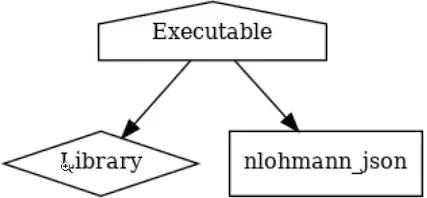
\includegraphics[width=2in]{graph.png}
\end{center}

\begin{center}
    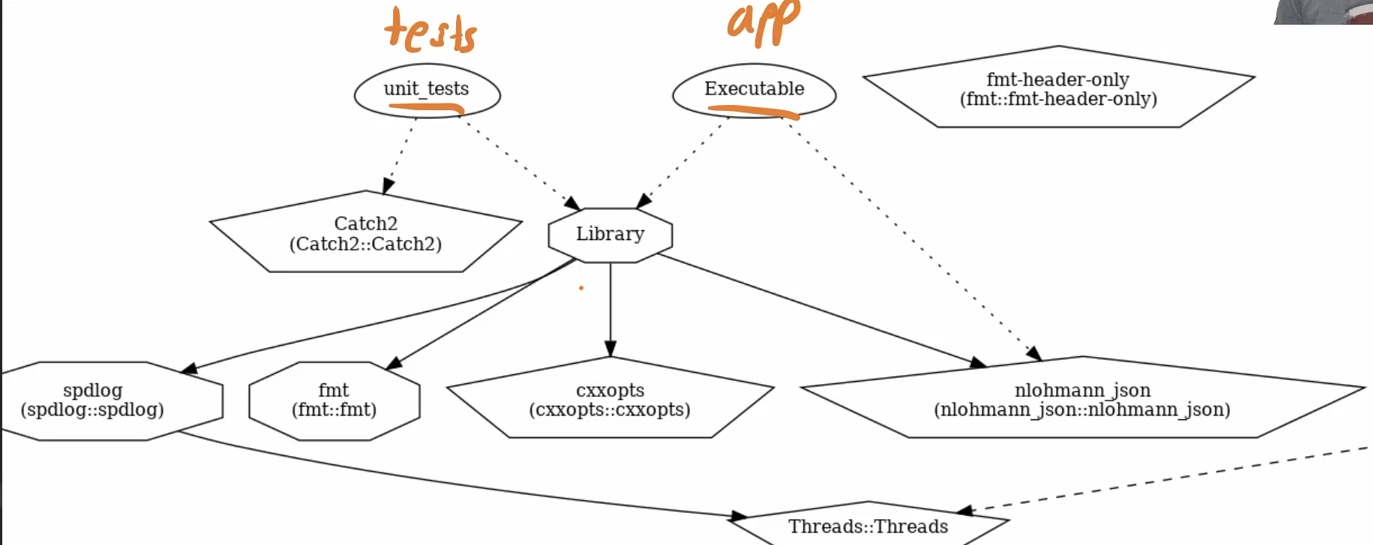
\includegraphics[width=6in]{graph3.png}
\end{center}

\section{Doxygen Documentation}

Generate html documentation for our code. For example, for our library. The course has a vscode extention: Doxygen Documentation Generator.

\subsection{Doxygen Vscode Extension}

The extention generates documentation base on this synthax.

\begin{verbatim}
#include <iostream>

#include <nlohmann/json.hpp>
#include "my_lib.h"

/**
 * @brief Prints out hello world and tests the JSON lib.
 *
 *
 */
\end{verbatim}

\subsection{Doxygen Command Line}

Doxygen is looking for a doxy file, a config file. Generate a doxy file with doxygen -g.
In it, fill information on the project, name, version,  path to source files, etc. It will generate better html file with the information.
In the docs directory.

\begin{center}
    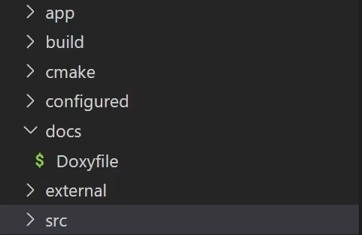
\includegraphics[width=2in]{dox.png}
\end{center}

\begin{verbatim}
# Configuration for Doxygen for use with CMake
# Only options that deviate from the default are included
# To create a new Doxyfile containing all available options, call `doxygen -g`

#---------------------------------------------------------------------------
# Project related configuration options
#---------------------------------------------------------------------------
DOXYFILE_ENCODING       = UTF-8
PROJECT_NAME            = "C++ Project Template"
PROJECT_NUMBER          = 1.0
PROJECT_BRIEF           =
PROJECT_LOGO            =
OUTPUT_DIRECTORY        = ./
OUTPUT_LANGUAGE         = English
MARKDOWN_SUPPORT        = YES

#---------------------------------------------------------------------------
# Build related configuration options
#---------------------------------------------------------------------------
EXTRACT_ALL             = YES
RECURSIVE               = YES
GENERATE_HTML           = YES
GENERATE_LATEX          = NO

#---------------------------------------------------------------------------
# Configuration options related to the input files
#---------------------------------------------------------------------------
INPUT                  =    ../src \
INPUT                       ../include
INPUT_ENCODING         = UTF-8
FILE_PATTERNS          = *.c \
                         *.cc \
                         *.cpp \
                         *.c++ \
                         *.h \
                         *.hpp \
                         *.h++ \
                         *.md \
                         *.dox \
                         *.doc \
                         *.txt
\end{verbatim}

When ready, generate the html with the command Doxygen, inside the docs folder (where the doxyfile is located). It creates an html dir.
it has the index.html automatically. The webpage looks like this:


\begin{center}
    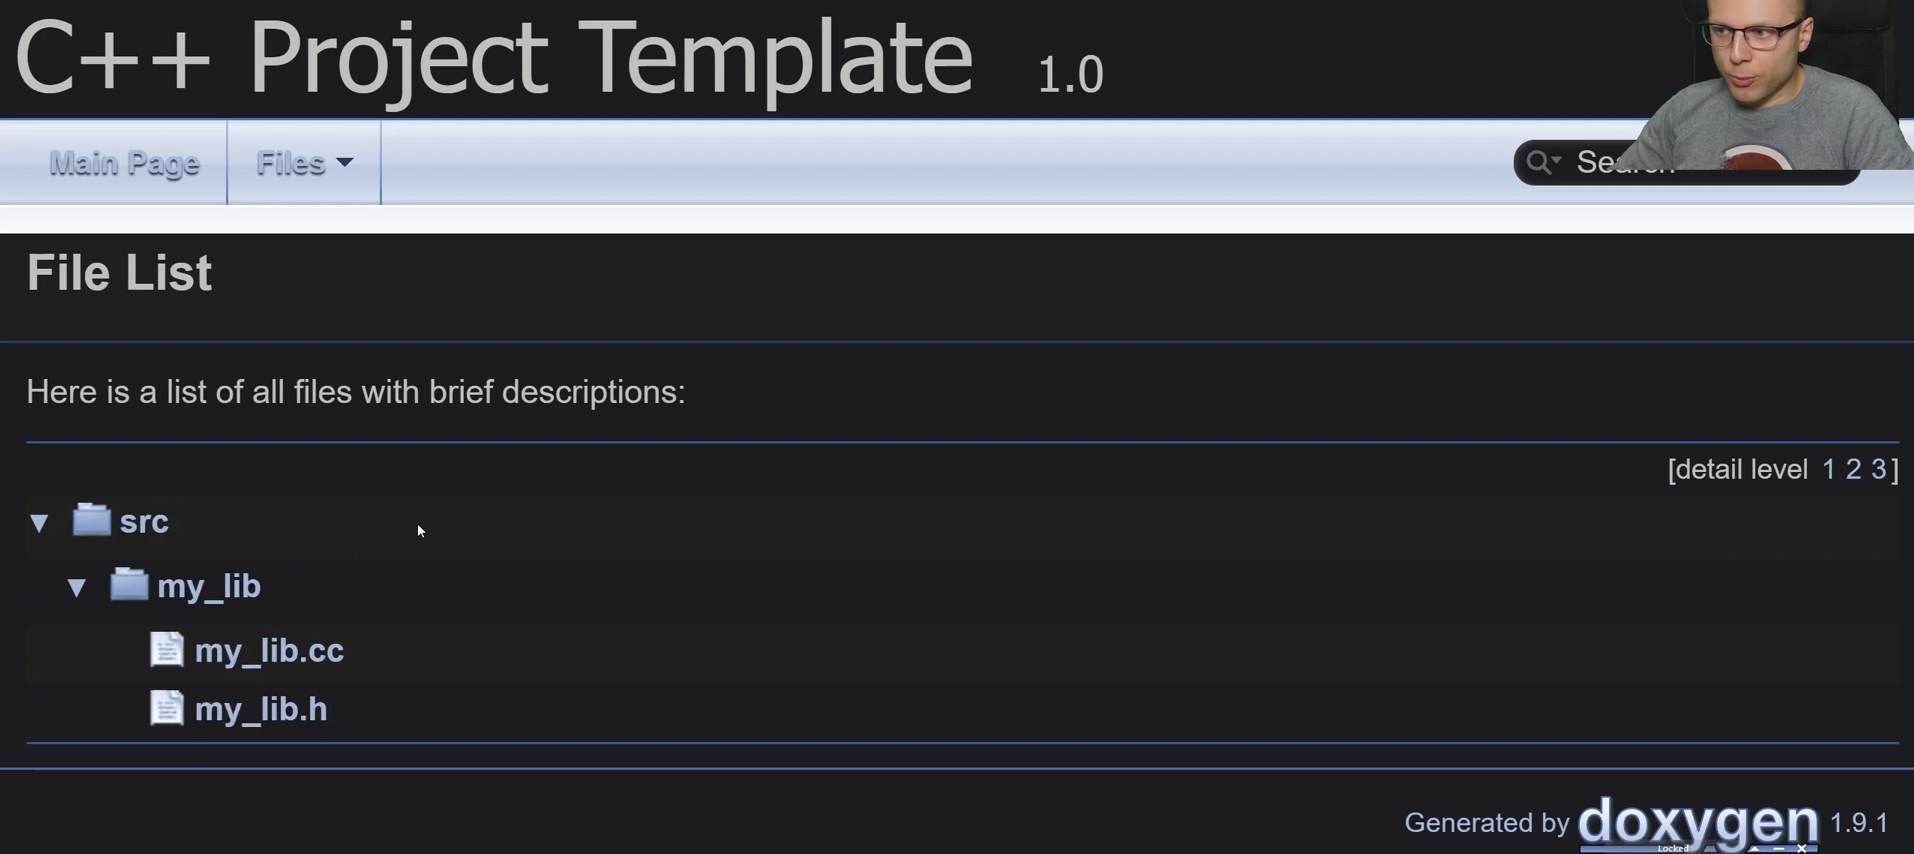
\includegraphics[width=5in]{dox2.png}
\end{center}


\subsection{Doxygen Custom Target Documentation}

We need to add the documentation to our cmake project.

\begin{center}
    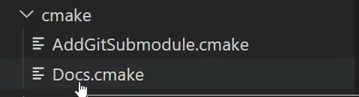
\includegraphics[width=3in]{doccmake.png}
\end{center}

In our root CMakeLists.txt, we add.

\begin{verbatim}
include(AddGitSubmodule)
include(FetchContent)
include(Docs)               # this is our new dir.

\end{verbatim}


\subsection{Doxygen Doc.cmake}

Cmake needs to find Doxygen, because we are using it for our docs. In Docs.cmake,

\begin{verbatim}
find_package(Doxygen)
if (DOXYGEN_FOUND)
    add_custom_target( # This is just an utility target
                       # With it, we can interact with it, 
                       # in the terminal
    docs
    ${DOXYGEN_EXECUTABLE}
    WORKING_DIRECTORY ${CMAKE_SOURCE_DIR}/docs

                       # CMAKE_SOURCE_DIR is always the directory of the
                       # root CMakeLIsts.txt file
                       # our root directory

                       # CMAKE_BINARY_DIR is always our build directory
endif()
\end{verbatim}

Now Documentation can be built seperately, independently of the main project app built process.

\section{Unit Testing in CMake}

\subsection{Catch2 - Function Unit Testing}

Adding Unit test to our codebase, with the catch2 library. Unit tests are useful to test functions from the library.

There is a tutorial on the github catch2 page. As an example, it provides this factorial function example, to try.

\begin{verbatim}
unsigned int factorial( unsigned int number ) {
    return number <= 1 ? number : factorial(number-1)*number;
}

// the instructor changes it to

std::uint32_t factorial(std::unint32_t number)
{
    return number <= 1 ? number : factorial(number-1) * number;
}
\end{verbatim}

\subsection{Unit Test Directory}

To introduce unit testing, we create a new directory: tests.

\begin{center}
    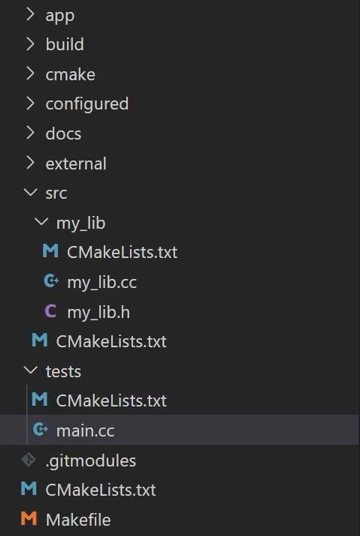
\includegraphics[width=2in]{tests.png}
\end{center}

In our root CMakeLists.txt.  

\begin{verbatim}
add_subdirectory(configured)
add_subdirectory(external)
add_subdirectory(src)
add_subdirectory(app)
add_subdirectory(tests) # adding tests
\end{verbatim}

\textbf{The idea is to have our main executable, our library(lib) and our unit test executable. The main and the Unit
executable we'll both use our library, but we will test with Unit. Unit will test if all our implemented functions work without bugs.}


\subsection{Unit Tests Configuration CMakeLists.txt}

\begin{verbatim}
set(TEST_MAIN "unit_tests")        # this is the name of our testing executable
set(TEST_SOURCES "main.cpp")       # Here, the tests are in one file only
                                   # It could be divided into more files
                                   # Header files for example
set(TEST_INCLUDES "./")
add_executable(${TEST_MAIN} ${TEST_SOURCES})
target_include_directories(${TEST_MAIN} PUBLIC ${TEST_INCLUDES})
target_link_libraries(${TEST_MAIN} PUBLIC ${LIBA} Catch2::Catch2)

                                   # Our library is linked, LIBA
                                   # This is how we will test it
\end{verbatim}


\subsection{Unit Tests Definition}

To test the factorial function, this is the test definition given as example.

\begin{verbatim}
#define CATCH_CONFIG_MAIN // This tells Catch to provide a main() - only do this in one file
                          // No need to write int main() {}, this does it. 
#include "catch2/catch.hpp"

#include "my_lib.h"       // Will be called in my_lib.h

TEST_CASE( "Factorials are computed", "[factorial]" ) {
    REQUIRE( Factorial(1) == 1);
    REQUIRE( Factorial(2) == 2);
    REQUIRE( Factorial(3 == 6);
    REQUIRE( Factorial(10 == 362880 );
}

This function needs to be called in my_lib.h

std::uint32_t factorial(std::uint32_t number);
\end{verbatim}


\subsection{Unit Testing Command Line Options}

It is convenient to have a command line option to activate or deactivate our testing build. In our root CMakeLists.txt
file, we add an option. In our CMakeLists.txt in the tests directory, we add an if statement. 

\begin{verbatim}
option(ENABLE_TESTING "Enable a Unit Testing Build" ON) 

# in tests directory's CMakeLists.txt

if (ENABLE_TESTING)
    set(TEST_MAIN "unit_tests")
    set(TEST_SOURCES "main.cpp")
    set(TEST_INCLUDES "./")

    add_executable(#{TEST_MAIN} ${TEST_SOURCES})
    target_include_directories(${TEST_MAIN} PUBLIC ${TEST_INCLUDES})
    target_link_libraries(${TEST_MAIN} PUBLIC ${LIBA} Catch2::Catch2)
endfi()
\end{verbatim}

\section{Linking Types Differences} 

Public and private is similar to OOP public and private keywords in classes.

\begin{verbatim}
add_library(A ...)
add_library(B ...)
add_library(C ...)
\end{verbatim}

\subsection{Linking Type Public}

Here, fmt can be used in the library of A. 

\begin{verbatim}
target_link_libraries(A PUBLIC fmt)

target_link_libraries(C PUBLIC/PRIVATE A)
target_link_libraries(C PUBLIC/PRIVATE A)
\end{verbatim}

When A links fmt as PUBLIC, it says that A uses fmt in its implementation, and fmt is also used in A's public API.
Hence, C can use fmt since it is part of the public API of A.

\subsection{Linking Type Private}

Using PRIVATE does not make the library available in the target's public API. Instead, it is part of a private API.
When B links in spdlog as PRIVATE, it is saying that B uses spdlog in its implementation,
but spdlog is not used in any part of B's public API. 

\begin{verbatim}
target_link_libraries(B PRIVATE spdlog)

target_link_libraries(C PUBLIC/PRIVATE B)
\end{verbatim}

Any code that makes calls into B would not need to refer directly to anything from
spdlog.


In a professional setting, you want to keep certain aspect of you project private. Hence, this option to consider.

\subsection{Linking Type Interface}

In general, used for header-only libraries. That is, libraries where you don't need to compile anything. They do not have
any compilation logic in them.

\begin{verbatim}
add_library(D INTERFACE)
target_include_directories(D INTERFACE {CMAKE_CURRENT_SOURCE_DIR}/include)

# this only links something to the executable, I think. No compilation logic.
\end{verbatim}


\section{Library Types Difference}

\subsection{Library Type Library}

A binary file that contains information about code.
A library cannot be executed on its own.
An application utilizes a library.

A library must be build too, if it is used by an executable.

\begin{verbatim}
cmake --build . --target Library
cmake --build . --target Executable // it is dependent to the Library build!
\end{verbatim}

\subsection{Library Type Shared}

\begin{verbatim}
Linux: *.so
MacOS: *.dylib
Windows: *.dll
\end{verbatim}

Shared libraries reduce the amount of code that is duplicated in each program that makes use of the library, keeping the binaries small.
Shared libraries will however have a small additional cost for the execution.
In general the shared library is in the same directory as the executable.

A file that needs to be carried along with the executable.

\begin{center}
    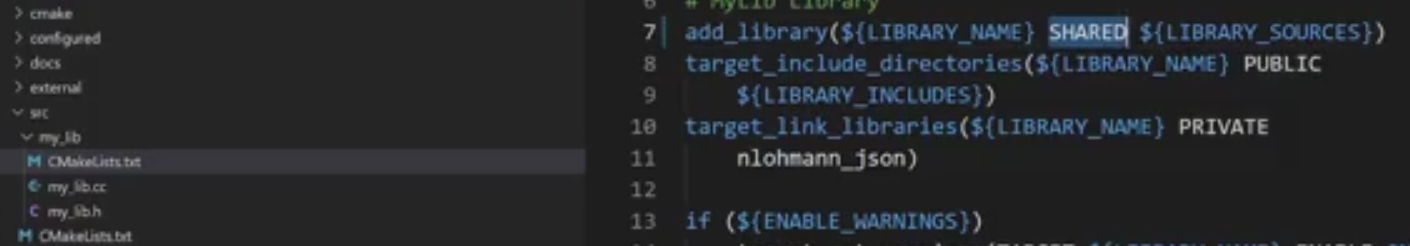
\includegraphics[width=2in]{shar.png}
\end{center}


\subsection{Library Type Static}

\begin{verbatim}
Linux/MacOS: *.a
Windows: *.lib
\end{verbatim}

Static libraries increase the overall size of the binary, but it means that you don't need to carry along a copy of the library that is being used.
As the code is connected at compile time there are not any additional run-time loading costs.

A staticly compiled into the executable.


\section{Compiler Warnings}

You can pull certain warnings for a particular target.
We can activate them based on the operating system and on the compiler.
We can trigger certain set of compiler checks.
In this course, we had two targets: the library target and the executable target.

In the cmake directory, add Warnings.cmake. 

\begin{center}
    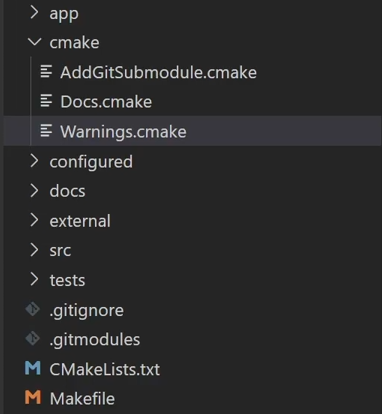
\includegraphics[width=2in]{warnings1.png}
\end{center}

\begin{verbatim}
function(target_set_warnings)
    set(oneValueArgs TARGET ENABLE AS_ERRORS)
    cmake_parse_arguments(
        TARGET_SET_WARNINGS             # every option and oneValueArgs
                                        # will be prefixed by
                                        # TARGET_SET_WARNINGS


                                        # this function was updated at the end of the course.
                                        # refactoring at the end of the course was hard to follow.
        "${options}"
        "${oneValueArgs}"
        "${multiValueArgs}"
        ${ARGN})

    if (NOT ${TARGET_SET_WARNINGS_ENABLE})
        message(STATUS "Warnings disabled for: ${TARGET_SET_WARNINGS_TARGET}")
        return()
    endif()
    message(STATUS "Warnings Active for: ${TARGET_SET_WARNINGS_TARGET}")
    message(STATUS "Warnings as Errors: ${TARGET_SET_WARNINGS_AS_ERRORS}")

    set(MSCV_COMPILER
        /WA4
        /permissive-)

    set(CLANG_COMPILER
        -Wall
        -Wextra
        -Wpedantic)

    set(GCC_WARNINGS ${CLANG_WARNINGS})

    if(${ENABLED_AS_ERRORS}}
        set(MSCV_WARNINGS ${MSVC_WARNINGS} /WX) # We need to append to our MSVC compiler
                                                # We append /WX

        set(CLANG_WARNINGS ${CLANG_WARNINGS} -Werror)
                                                # We append -Werror
        set(GCC_WARNINGS ${GCC_WARNINGS} -Werror)
    endif()

    if(CMAKE_CXX_COMPILER_ID MATCHES "MSVC")
        set(WARNINGS ${MSVC_WARNINGS})
    elseif(CMAKE_CXX_COMPILER_ID MATCHES "CLANG")
        set(WARNINGS ${CLANG_WARNINGS})
    elseif(CMAKE_CXX_COMPILER_ID MATCHES "GNU")
        set(WARNINGS ${GCC_WARNINGS})
    endif()

    target_compile_options(${TARGET} PRIVATE ${WARNINGS})
    message(STATUS ${WARNINGS})

endfunction(target_set_warnings TARGET)
\end{verbatim}

\subsection{Compiler Check User's Compiler}

\begin{verbatim}
if(CMAKE_CXX_COMPILER_ID MATCHES "MSVC")
    set(WARNINGS ${MSVC_WARNINGS})
elseif(CMAKE_CXX_COMPILER_ID MATCHES "CLANG")
    set(WARNINGS ${CLANG_WARNINGS})
elseif(CMAKE_CXX_COMPILER_ID MATCHES "GNU")
    set(WARNINGS ${GCC_WARNINGS})
endif()
\end{verbatim}


\subsection{Compiler Warnings Root CMakeLists Options}

We just created a function to check the user's compiler and set compilation warnings.
Now create options in the root CMakeFilelists.txt.

\begin{verbatim}
option(ENABLE_WARNINGS "Enable warnings" ON)
option(ENABLE_WARNINGS_AS_ERRORS "Enable warnings as errors" ON)

    ...

if(ENABLE_WARNINGS)
    include(Warnings) # include the newly created Warnings.cmake file
endif()
\end{verbatim}


\subsection{Compiler Warnings Executable Target}

There are two targets that can have compilation warnings, our library and our executable (our app). We have to 
add warning conditionals in both of their CMakeLists.txt file.

\begin{verbatim}
if(${ENABLE_WARNINGS})
    target_set_warnings(
        ${HE}       # this is our executable / app name,
                    # passed as argument in our created warnings function
        ${ENABLE_WARNINGS}
        ${ENABLE_WARNINGS_AS_ERRORS})
endif()

# for the lib CMakeLists.txt

if(${ENABLE_WARNINGS})
    target_set_warnings(
        ${LIBA}       # this is our library target name,
                      # passed as argument in our created warnings function
        ${ENABLE_WARNINGS}
        ${ENABLE_WARNINGS_AS_ERRORS})
endif()
\end{verbatim}

You don't have to have warnings as error for all targets, but you should have compilation warnings for all of them.

\section{Sanitizers}

Use sanitizers to find memory links or memory problems in your code. Sanitizers are used at runtime. 
Thus, it happens after compilation. Clang-tidy is a static linter, it finds problems before compilation!  

In order, you have clang-tidy before compilation, 
compiler warnings during compilation and sanitizers at runtime (after compilation).

In our root CMakeLists.txt, we add

\begin{verbatim}
option(ENABLE_SANITIZE_ADDR "Enable warnings" ON)
option(ENABLE_SANITIZE_UNDEF "Enable warnings" ON)


if(ENABLE_SANITIZE_UNDUF OR ENABLE_SANITIZE_ADDR)
    include(Sanitizers) # include a Sanitizers.cmake file
                        # same as Warnings.cmake file
endif()

\end{verbatim}

\begin{center}
    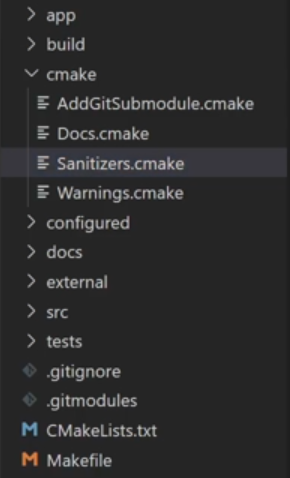
\includegraphics[width=2in]{san.png}
\end{center}


\subsection{Sanitizers.cmake}

In cmake directory, we have this file.


\begin{verbatim}
function(add_sanitizer_flags)
    if(NOT ${ENABLE_SANITIZE_UNDEF} AND NOT ${ENABLE_SANITIZE_ADDR})
        message(STATUS "Sanitizers deactivated") 
        return()
    endif()

    if(CMAKE_CXX_COMPILER_ID MATCHES "CLANG" OR CMAKE_CXX_COMPILER_ID MATCHES "GNU")
        add_compile_options("-fno-omit-frame-pointer")   
                                        # This functions adds compiler flags for every target
                                        # Sanitizers need to run on all of the application
        add_link_options("-fno-omit-frame-pointer")

        if (${ENABLE_SANITIZE_ADDR})
            add_compile_options("-fsanitize=address") 
            add_link_options("-fsanitize=address") 
        endif()

        if (${ENABLE_SANITIZE_UNDEF})
            add_compile_options("-fsanitize=undefined") 
            add_link_options("-fsanitize=undefined") 
        endif()

    elseif(CMAKE_CXX_COMPILER_ID MATCHES "MSVC")
        if (${ENABLE_SANITIZE_ADDR})
            add_compile_options("-fsanitize=address") 
            add_link_options("-fsanitize=address") 
        endif()

        if (${ENABLE_SANITIZE_UNDEF})
            message(STATUS "Undefined sanitizer is not implemented for MVSC")
        endif()

    else() 
        message(ERROR "Compiler not supported for Sanitizers")
    endif()
endfunction()
\end{verbatim}


\subsection{Sanitizers Activation in Root CMakeLists.txt}

Call the add\_sanitizer\_flags function from root.

\begin{verbatim}
if(ENABLE_SANITIZE_ADDR OR ENABLE_SANITIZE_UNDEF)
    include(Sanitizers)
    add_sanitizer_flags()
endif()
\end{verbatim}

\subsection{Sanitizer Bugs}

Going out of bounds, like this, would be caught be clang-tidy, but not by compilers. Thus, Sanitizers help big time. See documentation at
gcc.gnu.org/onlinedocs/Instrumentation-Options.html.


\begin{center}
    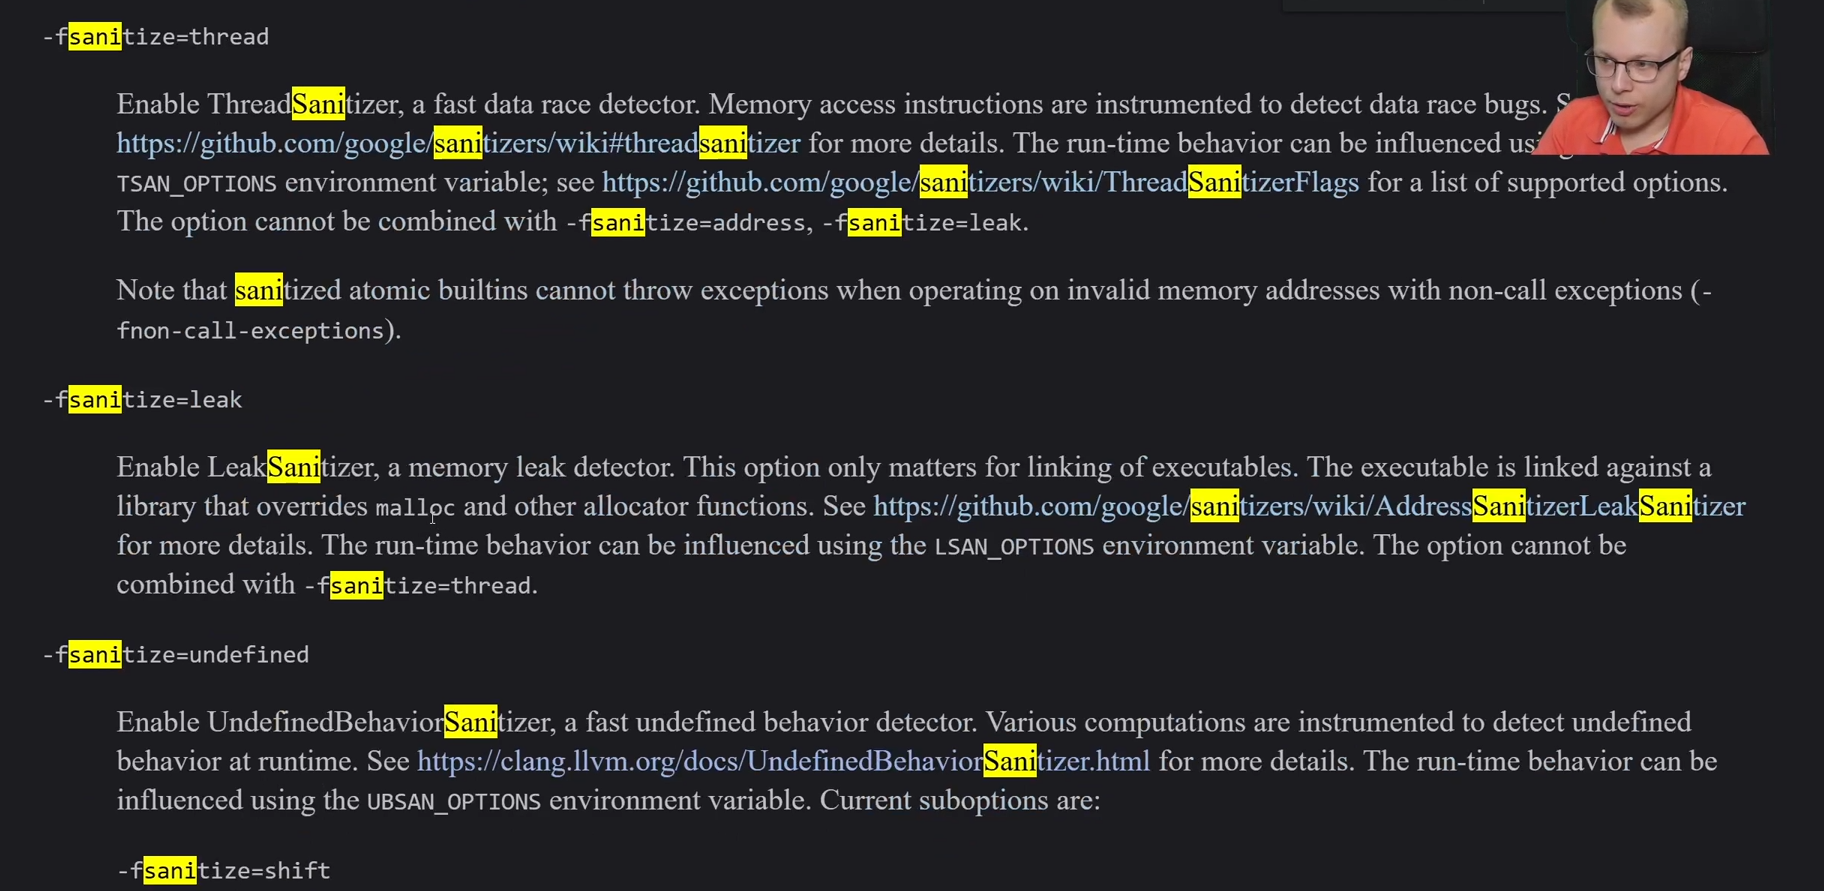
\includegraphics[width=5in]{fsan.png}
\end{center}


\begin{verbatim}
int main() {
    int x[2];
    x[2] = 1337;
}
\end{verbatim}

\section{IPO LTO}

In release mode, the release build, optimizations are activated to create the best product. C++ has many types of builds
for a project, debug modes, performance modes, etc. 

In this case, the release mode optimizations are related to the compiler for a better runtime. Yet, these optimizations
look at functions separately, not as a chain of functions so to speak (subsequent calls of different functions).

Link Time Optimization (LTO) or Interprocedural Optimization (IPO) [synonyms] is a response to these limits. Using functions from different translation units, the compiler with optimizations,
will be able to analyse them subsequently. In other words, the optimized compiler will be able to evaluate
if some operations can be cancelled in the function chain.

To use it, we will use a CMake function. All compilers (MSVC, CLANG and GCC) have LTO implemented.


\subsection{LTO Example - Clang}

\begin{verbatim}
--- a.h --- // .h for header file
            // this is genius note-taking!!!

extern int foo1(void);
extern void foo2(void);
extern void foo4(void);

--- a.c --- // .c for source file
            // this is genius note-taking!!!

#include "a.h"

static signed int i = 0;

void foo2(void {
    i = -1; 
}

static int foo3(void {
    i = -1; 
}

int foo1(void) {
    int data = 0;

    if (i < 0)
        data = foo3();

    data = data + 42;
    return data;
}

--- main.c ---
#include <stdio.h>
#include "a.h"

void foo4(void){
    printf("Hi\n");
}

int main() {
    return foo1()
}
\end{verbatim}

In this example, it is impossible for i to be reduced under zero. Since it is impossible, the foo3 function will never be
called. Thus, the compiler cancels an impossible chain and does not generate code for these logically uncallable functions.
This is the optimization.

\subsection{IPO LTO in CMake}

In your cmake directory, create a LTO.cmake file. Plus, create a new option in your root CMakelists.txt


\begin{verbatim}
option(ENABLE_LTO "Enable the link time optimization" ON)

...

if(ENABLE_LTO)
    include(LTO)
endif()
\end{verbatim}


\subsection{LTO.cmake}

Configuring link time optimization in the new lto.cmake file, in the cmake directory.

\begin{verbatim}
function(target_enable_lto TARGET ENABLE)
    if(NOT ${ENBALE})
    endif()

    include(CheckIPOSupported)
    check_ipo_supported(RESULT result OUTPUT output)

    if(result) 
        message(STATUS "IPO/LTO is supported!")
        set_property(TARGET ${TARGET} PROPERTY_INTERPROCEDURAL_OPTIMIZATION ${ENABLE})
    else()
        message("WARNING "IPO/LTO is not supported!")

                                     #PROPERTY... is a predefined variable in modern cmake
    endif()
endfunction(target_enable_lto)
\end{verbatim}

\subsection{LTO.cmake Refactoring}

The instructor revised the lto.cmake file at the end of the course.

\begin{verbatim}
function(target_enable_lto)         # he passes less arguments here
    set(oneValueArgs TARGET ENABLE)
    cmake_parse_arguments(          # every options and arguments in oneValueArgs
                                    # will be prefixed by LTO_
                                    # thus, TARGET becomes LTO_TARGET
        LTO
        "${options}"
        "${oneValueArgs}"
        "${multiValueArgs}"
        ${ARGN})


    include(CheckIPOSupported)
    check_ipo_supported(RESULT result OUTPUT output)

    if(result) 
        message(STATUS "IPO/LTO is supported: ${LTO_TARGET}")
        set_property(TARGET ${LTO_TARGET} PROPERTY_INTERPROCEDURAL_OPTIMIZATION ${LTO_ENABLE})
    else()
        message("WARNING "IPO/LTO is not supported! ${LTO_TARGET}")

                                     #PROPERTY... is a predefined variable in modern cmake
    endif()
endfunction(target_enable_lto)
\end{verbatim}

\subsection{In Our Target CMakeLists.txt}

Enabling LTO for our target library, means configuring it in its CMakeLists.txt file.

\begin{center}
    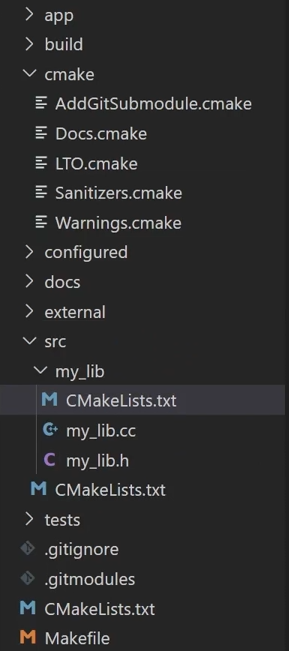
\includegraphics[width=2in]{lto_lib.png}
\end{center}


\begin{verbatim}
if(${ENABLE_LTO})
    target_enable_lto(${LIBRARY_NAME})
endif()

---- in app ----
---- CMakeLists.txt ----

if(${ENABLE_LTO})
    target_enable_lto(${EXECUTABLE_NAME} ${ENABLE_LTO})
endif()
\end{verbatim}

\chapter{Clang Tools}

\section{Clang Tools.cmake}

Configure the tools in a new Tools.cmake file.

\begin{center}
    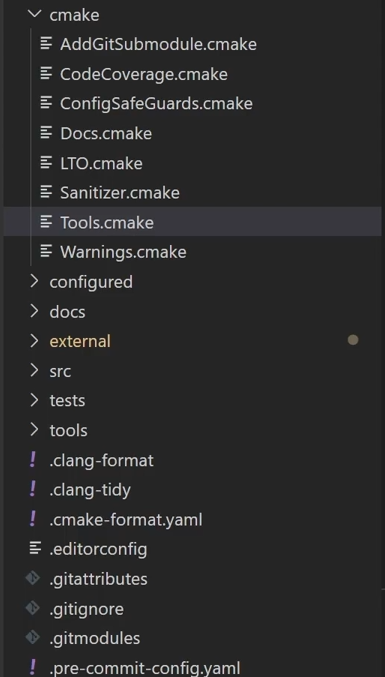
\includegraphics[width=2in]{tools_cm.png}
\end{center}


\begin{verbatim}
function(add_cmake_format_target)
    if(NOT ${ENABLE_CMAKE_FORMAT})
        return()
    endif()
    set(ROOT_CMAKE_FILES "${CMAKE_SOURCE_DIR}/CMakeLists.txt")
    file(GLOB_RECURSE CMAKE_FILES_TXT "*/CMakeLists.txt")
    file(GLOB_RECURSE CMAKE_FILES_C "cmake/*.cmake")
    list(
        FILTER
        CMAKE_FILES_TXT
        EXCLUDE
        REGEX
        "${CMAKE_SOURCE_DIR}/(build|external)/.*")
    set(CMAKE_FILES ${ROOT_CMAKE_FILES} ${CMAKE_FILES_TXT} ${CMAKE_FILES_C})
    find_program(CMAKE_FORMAT cmake-format)
    if(CMAKE_FORMAT)
        message(STATUS "Added Cmake Format")
        set(FORMATTING_COMMANDS)
        foreach(cmake_file ${CMAKE_FILES})
            list(
                APPEND
                FORMATTING_COMMANDS
                COMMAND
                cmake-format
                -c
                ${CMAKE_SOURCE_DIR}/.cmake-format.yaml
                -i
                ${cmake_file})
        endforeach()
        add_custom_target(
            run_cmake_format
            COMMAND ${FORMATTING_COMMANDS}
            WORKING_DIRECTORY ${CMAKE_SOURCE_DIR})
    else()
        message(WARNING "CMAKE_FORMAT NOT FOUND")
    endif()
endfunction()

function(add_clang_format_target)
    if(NOT ${ENABLE_CLANG_FORMAT})
        return()
    endif()
    find_package(Python3 COMPONENTS Interpreter)
    if(NOT ${Python_FOUND})
        return()
    endif()
    file(GLOB_RECURSE CMAKE_FILES_CC "*/*.cc")
    file(GLOB_RECURSE CMAKE_FILES_CPP "*/*.cpp")
    file(GLOB_RECURSE CMAKE_FILES_H "*/*.h")
    file(GLOB_RECURSE CMAKE_FILES_HPP "*/*.hpp")
    set(CPP_FILES
        ${CMAKE_FILES_CC}
        ${CMAKE_FILES_CPP}
        ${CMAKE_FILES_H}
        ${CMAKE_FILES_HPP})
    list(
        FILTER
        CPP_FILES
        EXCLUDE
        REGEX
        "${CMAKE_SOURCE_DIR}/(build|external)/.*")
    find_program(CLANGFORMAT clang-format)
    if(CLANGFORMAT)
        message(STATUS "Added Clang Format")
        add_custom_target(
            run_clang_format
            COMMAND
                ${Python3_EXECUTABLE}
                ${CMAKE_SOURCE_DIR}/tools/run-clang-format.py ${CPP_FILES}
                --in-place
            WORKING_DIRECTORY ${CMAKE_SOURCE_DIR}
            USES_TERMINAL)
    else()
        message(WARNING "CLANGFORMAT NOT FOUND")
    endif()
endfunction()

function(add_clang_tidy_to_target target)
    get_target_property(TARGET_SOURCES ${target} SOURCES)
    list(
        FILTER
        TARGET_SOURCES
        INCLUDE
        REGEX
        ".*.(cc|h|cpp|hpp)")

    find_package(Python3 COMPONENTS Interpreter)
    if(NOT ${Python_FOUND})
        message(WARNING "Python3 needed for Clang-Tidy")
        return()
    endif()

    find_program(CLANGTIDY clang-tidy)
    if(CLANGTIDY)
        if(CMAKE_CXX_COMPILER_ID MATCHES "MSVC")
            message(STATUS "Added MSVC ClangTidy (VS GUI only) for: ${target}")
            set_target_properties(
                ${target} PROPERTIES VS_GLOBAL_EnableMicrosoftCodeAnalysis
                                     false)
            set_target_properties(
                ${target} PROPERTIES VS_GLOBAL_EnableClangTidyCodeAnalysis true)
        else()
            message(STATUS "Added Clang Tidy for Target: ${target}")
            add_custom_target(
                ${target}_clangtidy
                COMMAND
                    ${Python3_EXECUTABLE}
                    ${CMAKE_SOURCE_DIR}/tools/run-clang-tidy.py
                    ${TARGET_SOURCES}
                    -config-file=${CMAKE_SOURCE_DIR}/.clang-tidy
                    -extra-arg-before=-std=${CMAKE_CXX_STANDARD}
                    -header-filter="\(src|app\)\/*.\(h|hpp\)"
                    -p=${CMAKE_BINARY_DIR}
                WORKING_DIRECTORY ${CMAKE_CURRENT_SOURCE_DIR}
                USES_TERMINAL)
        endif()
    else()
        message(WARNING "CLANGTIDY NOT FOUND")
    endif()
endfunction()
\end{verbatim}


\subsection{Clang Tool Directory}

The previous tool.cmake file references two python files, one for clang-format and one for clang-tidy.
Both are part of the LLVM package, no need to inspect those, it is part of the programs.

\begin{center}
    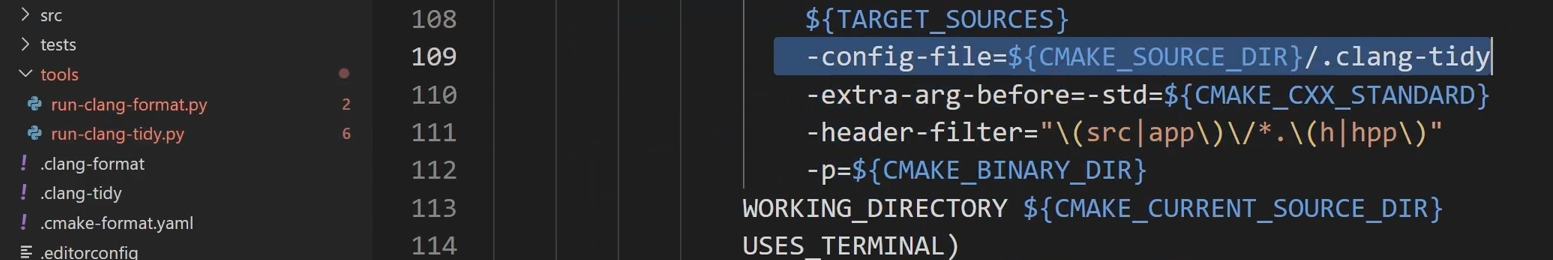
\includegraphics[width=6in]{runclang.png}
\end{center}

\subsection{Clang-Tidy}

A static linting tool for cpp, also known as static analyzers. It checks your code according
to set verifications. It is similar to compile warnings, but a linter does not require any compilation
to run. It checks to code whenever needed.


You do not need to use the clang compiler to use it.


It is nice to use, because it is the earliest form of warnings. It saves a ton of time if you do not have to compile
to have warnings. Early on is best.


\textbf{Use clang-tidy's modernize-loop-convert check} for range based loops.


\begin{verbatim}
Documentation for Clang-Tidy: https://clang.llvm.org/extra/clang-tidy/
\end{verbatim}


\subsection{.clang-tidy file}

Specify the checks clang-tidy executes in a .clang-tidy file at the root of your project.

\begin{verbatim}
Checks: 'clang-analyzer-*,cppcoreguidelines-*,
        modernize-*,bugprone-*,performance-*,readability-non-const-parameter,
        misc-const-correctness,misc-use-anonymous-namespace,
        google-explicit-constructor,-modernize-use-trailing-return-type,
        -bugprone-exception-escape,-cppcoreguidelines-pro-bounds-constant-array-index,
        -cppcoreguidelines-avoid-magic-numbers,-bugprone-easily-swappable-parameters'


        # modernize-* --------------- includes all warnings in this category
        # -bugprone=exception-escape # - with a '-' char, 
                                     # specifies one omition in the group

WarningsAsErrors: ''
HeaderFilterRegex: '\(src|app\)\/*.\(h|hpp\)'
AnalyzeTemporaryDtors: false
FormatStyle:     none
\end{verbatim}


\subsection{Clang-tidy Target}

Configuring a target for clang-tidy checks is made possible in the target's CMakeLists.txt. Here, in my\_lib dir
for library, our target.


\begin{verbatim}
if(${ENABLE_CLANG_TIDY})
    add_clang_tidy_to_target(${LIBA}) # this is defined in the Tools.cmake file
endif()
\end{verbatim}

\subsection{Clang-tidy in root CMakeLists.txt}

Create an option for clang-tidy in your projects' root CMakeLists.txt

\begin{verbatim}
option(ENABLE_CLANG_TIDY "Enable to add clang tidy." ON)


set(CMAKE_EXPOET_COMPILE_COMMANDS ON) # this cmake function creates a json file
                                      # clang-tidy needs this json to work
                                      # to differenciate your code from dependencies.

\end{verbatim}


\subsection{Clang-tidy on Microsoft MSVC}

To activate it with the microsoft compiler, you need to use the Visual Studio Code GUI only.
Some filters, defined in .clang-tidy config file may not work on Windows, but will work on Unix systems.

\begin{center}
    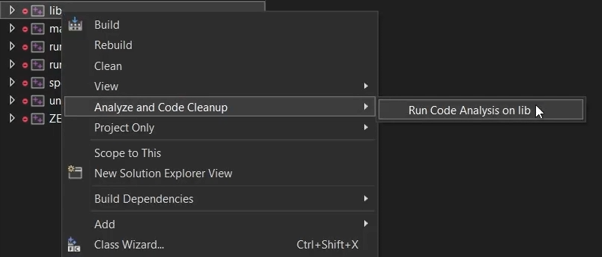
\includegraphics[width=5in]{ms_tidy.png}
\end{center}

 
\subsection{Clang-Format}

An essential professional formatting tool for cpp. Use version 14 at least, 16+ is best. The 
clang-tidy and clang-format .py files expects at least clang-format 14. Command line arguments 
change with versions. Check cpp project template .clang-format file in root directory.

Plus, these tools were configured in the root CMakeLists.txt file.

\begin{verbatim}
Documentation for Clang-Format: https://clang.llvm.org/docs/ClangFormat.html

Install Clang Tools

It's included in the LLVM toolchain, but also installable by apt, brew, winget etc.

https://github.com/llvm/llvm-project/releases/tag/llvmorg-16.0.0
\end{verbatim}


\subsection{Clang-Format Configuration in Tools.cmake}


\begin{verbatim}
function(add_clang_format_target)
    if(NOT ${ENABLE_CLANG_FORMAT})
        return()
    endif()
    find_package(Python3 COMPONENTS Interpreter)
    if(NOT ${Python_FOUND})
        return()
    endif()
    file(GLOB_RECURSE CMAKE_FILES_CC "*/*.cc")
    file(GLOB_RECURSE CMAKE_FILES_CPP "*/*.cpp")
    file(GLOB_RECURSE CMAKE_FILES_H "*/*.h")
    file(GLOB_RECURSE CMAKE_FILES_HPP "*/*.hpp")
    set(CPP_FILES
        ${CMAKE_FILES_CC}
        ${CMAKE_FILES_CPP}
        ${CMAKE_FILES_H}
        ${CMAKE_FILES_HPP})
    list(
        FILTER
        CPP_FILES
        EXCLUDE
        REGEX
        "${CMAKE_SOURCE_DIR}/(build|external)/.*") 

                                # exclude build and external files

    find_program(CLANGFORMAT clang-format)
    if(CLANGFORMAT)
        message(STATUS "Added Clang Format")
        add_custom_target(
            run_clang_format
            COMMAND
                ${Python3_EXECUTABLE}
                ${CMAKE_SOURCE_DIR}/tools/run-clang-format.py ${CPP_FILES}
                --in-place
            WORKING_DIRECTORY ${CMAKE_SOURCE_DIR}
            USES_TERMINAL)
    else()
        message(WARNING "CLANGFORMAT NOT FOUND")
    endif()
endfunction()
\end{verbatim}

\subsection{CMake-Format}

A nice-to-have .cmake file formater. It may make your project easier to read, 
since it standardizes all of your CMakeLists.txt files and .
Check .cmake-format.yaml file in root directory.

Plus, these tools were configured in the root CMakeLists.txt file.

\begin{center}
    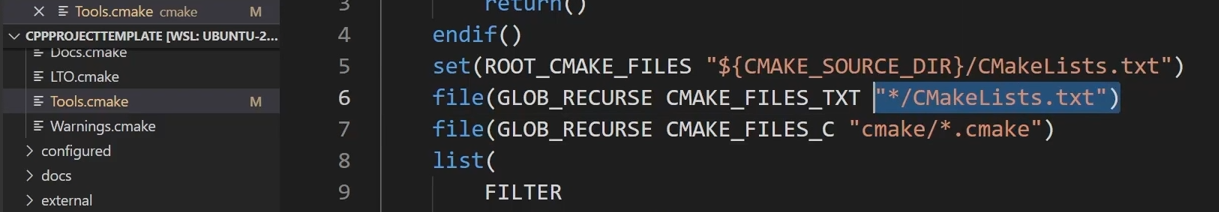
\includegraphics[width=5in]{tools4.png}
\end{center}


\begin{verbatim}
Install CMake-format,

pip install cmake-format # python 3.7+
\end{verbatim}


\subsection{CMake-Format Configuration in Tools.cmake}


\begin{verbatim}
function(add_cmake_format_target)
    if(NOT ${ENABLE_CMAKE_FORMAT})
        return()
    endif()
    set(ROOT_CMAKE_FILES "${CMAKE_SOURCE_DIR}/CMakeLists.txt")
    file(GLOB_RECURSE CMAKE_FILES_TXT "*/CMakeLists.txt")
    file(GLOB_RECURSE CMAKE_FILES_C "cmake/*.cmake")
    list(
        FILTER
        CMAKE_FILES_TXT
        EXCLUDE
        REGEX
        "${CMAKE_SOURCE_DIR}/(build|external)/.*")
    set(CMAKE_FILES ${ROOT_CMAKE_FILES} ${CMAKE_FILES_TXT} ${CMAKE_FILES_C})
    find_program(CMAKE_FORMAT cmake-format)
    if(CMAKE_FORMAT)
        message(STATUS "Added Cmake Format")
        set(FORMATTING_COMMANDS)
        foreach(cmake_file ${CMAKE_FILES})
            list(
                APPEND
                FORMATTING_COMMANDS
                COMMAND
                cmake-format
                -c                     # this flag finds the config flag. 
                                       # this is the file.
                ${CMAKE_SOURCE_DIR}/.cmake-format.yaml

                -i                     # specifies to replace the file in-place.
                                       # Otherwise, like sed command,
                                       # it only outputs the file
                ${cmake_file})
        endforeach()
        add_custom_target(
            run_cmake_format
            COMMAND ${FORMATTING_COMMANDS}
            WORKING_DIRECTORY ${CMAKE_SOURCE_DIR})
    else()
        message(WARNING "CMAKE_FORMAT NOT FOUND")
    endif()
endfunction()
\end{verbatim}

\subsection{Glob and Exclude Cmake Functions}

For clang and cmake-format tools, the tools.cmake file contains globing functions to
find all .cmake and CMakeLists.txt files.


\begin{center}
    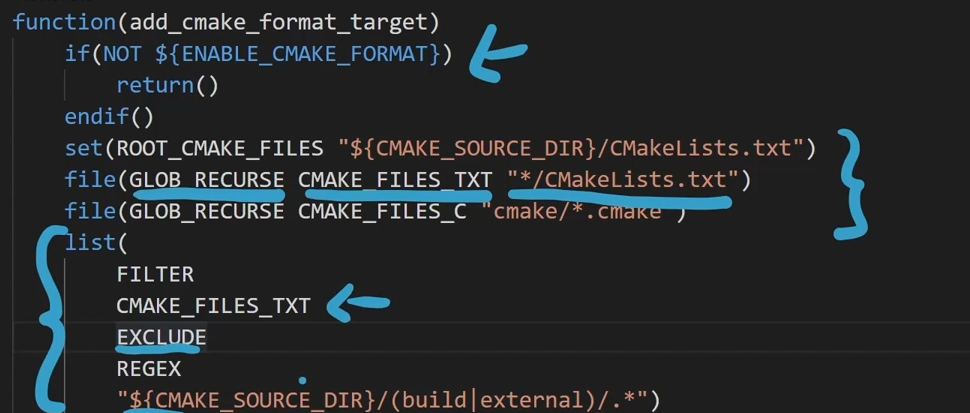
\includegraphics[width=2in]{glob.png}
\end{center}

\subsection{Github Pages}

Since Doxygen creates an html you can have a github-pages branch of your project and
use github pages to create a webpage your project.

In your .github directory of you project, in a workflows directory, create a documentation.yaml file. 
This will configure github to update your doc webpage automatically.


\begin{center}
    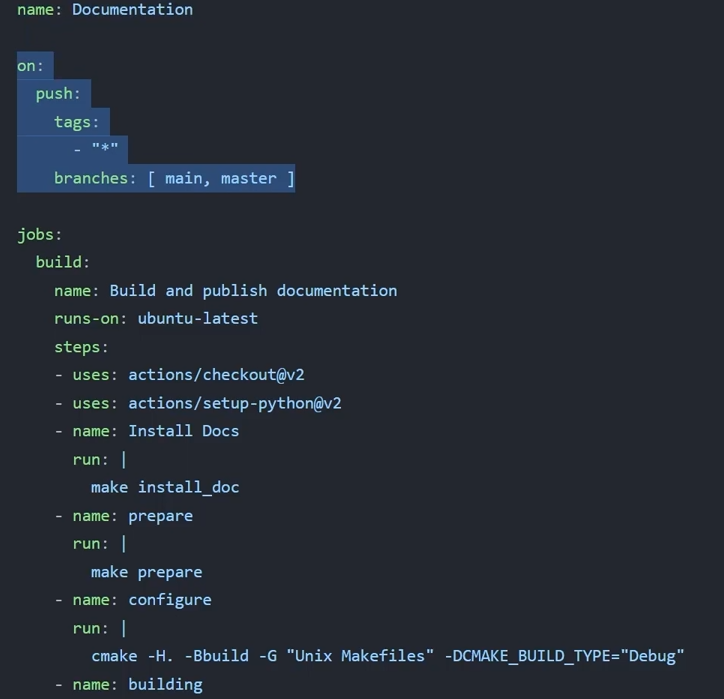
\includegraphics[width=2in]{pages.png}
\end{center}

Then, when we push to master, all the jobs will be run by github.

\begin{verbatim}
name: Documentation

on:
  push:
    tags:
      - "*"
    branches: [ main, master ]

jobs:
  build:
    name: Build and publish documentation
    runs-on: ubuntu-latest
    steps:
    - uses: actions/checkout@v2
    - uses: actions/setup-python@v2
    - name: Install Docs
      run: |
        sudo apt-get install doxygen
        pip install jinja2 Pygments
    - name: prepare
      run: |
        make prepare
    - name: configure
      run: |
        cmake -H. -Bbuild -G "Unix Makefiles" -DCMAKE_BUILD_TYPE="Debug"
    - name: building
      run: |
        cmake --build build --config Debug --target docs -j4
    - name: Deploy to GitHub Pages
      uses: Cecilapp/GitHub-Pages-deploy@v3
      env:
        GITHUB_TOKEN: ${{ secrets.GITHUB_TOKEN }}
      with:
        build_dir: ./docs/html   # where is the doxygen documentation
\end{verbatim}

It hosts the website on MikaelJG.github.io/repo-name/. Public documentation uploaded online.

\section{Code Coverage}

A metric to know how many lines of code were tested by our unit tests.
These tools are only available in linux.

\begin{verbatim}
sudo apt-get install gcovr lcov
\end{verbatim}

\subsection{Code Coverage Configuration in root CMakeLists.txt}

\begin{verbatim}
option(ENABLE_COVERAGE "Enable a Code COverage build." ON)

...

if(ENABLE_COVERAGE)
    include(CodeCoverage)
    append_coverage_compiler_flags() # defined in CodeCoverage.cmake file
endif()

\end{verbatim}

\subsection{Code Coverage for target library in my lib CMakeLists.txt}

Configure code coverage for a specific target in its CMakeLists.txt file.

\begin{verbatim}
if(ENABLE_COVERAGE)
    set(COVERAGE_MAIN "coverage") # the name of this coverage to run
    set(COVERAGE_EXCLUDES
        "${PROJECT_SOURCE_DIR}/app/*"
        "${PROJECT_SOURCE_DIR}/cmake/*"
        "${PROJECT_SOURCE_DIR}/docs/*"
        "${PROJECT_SOURCE_DIR}/external/*"
        "${PROJECT_SOURCE_DIR}/tests/*"
        "${PROJECT_SOURCE_DIR}/build/*"
        "$usr/indlude/*")
    setup_target_for_coverage_lcov(
        NAME
        ${COVERAGE_MAIN}
        EXECUTABLE
        ${UNIT_TEST_NAME}
        DEPENDENCIES
        ${UNIT_TEST_NAME})
endif()
\end{verbatim}


\subsection{Code Coverage Directory}

lcov generates a code Coverage directory, with information in an html.


\begin{center}
    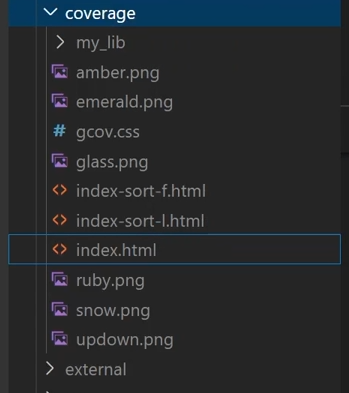
\includegraphics[width=2in]{cov.png}
\end{center}


\begin{center}
    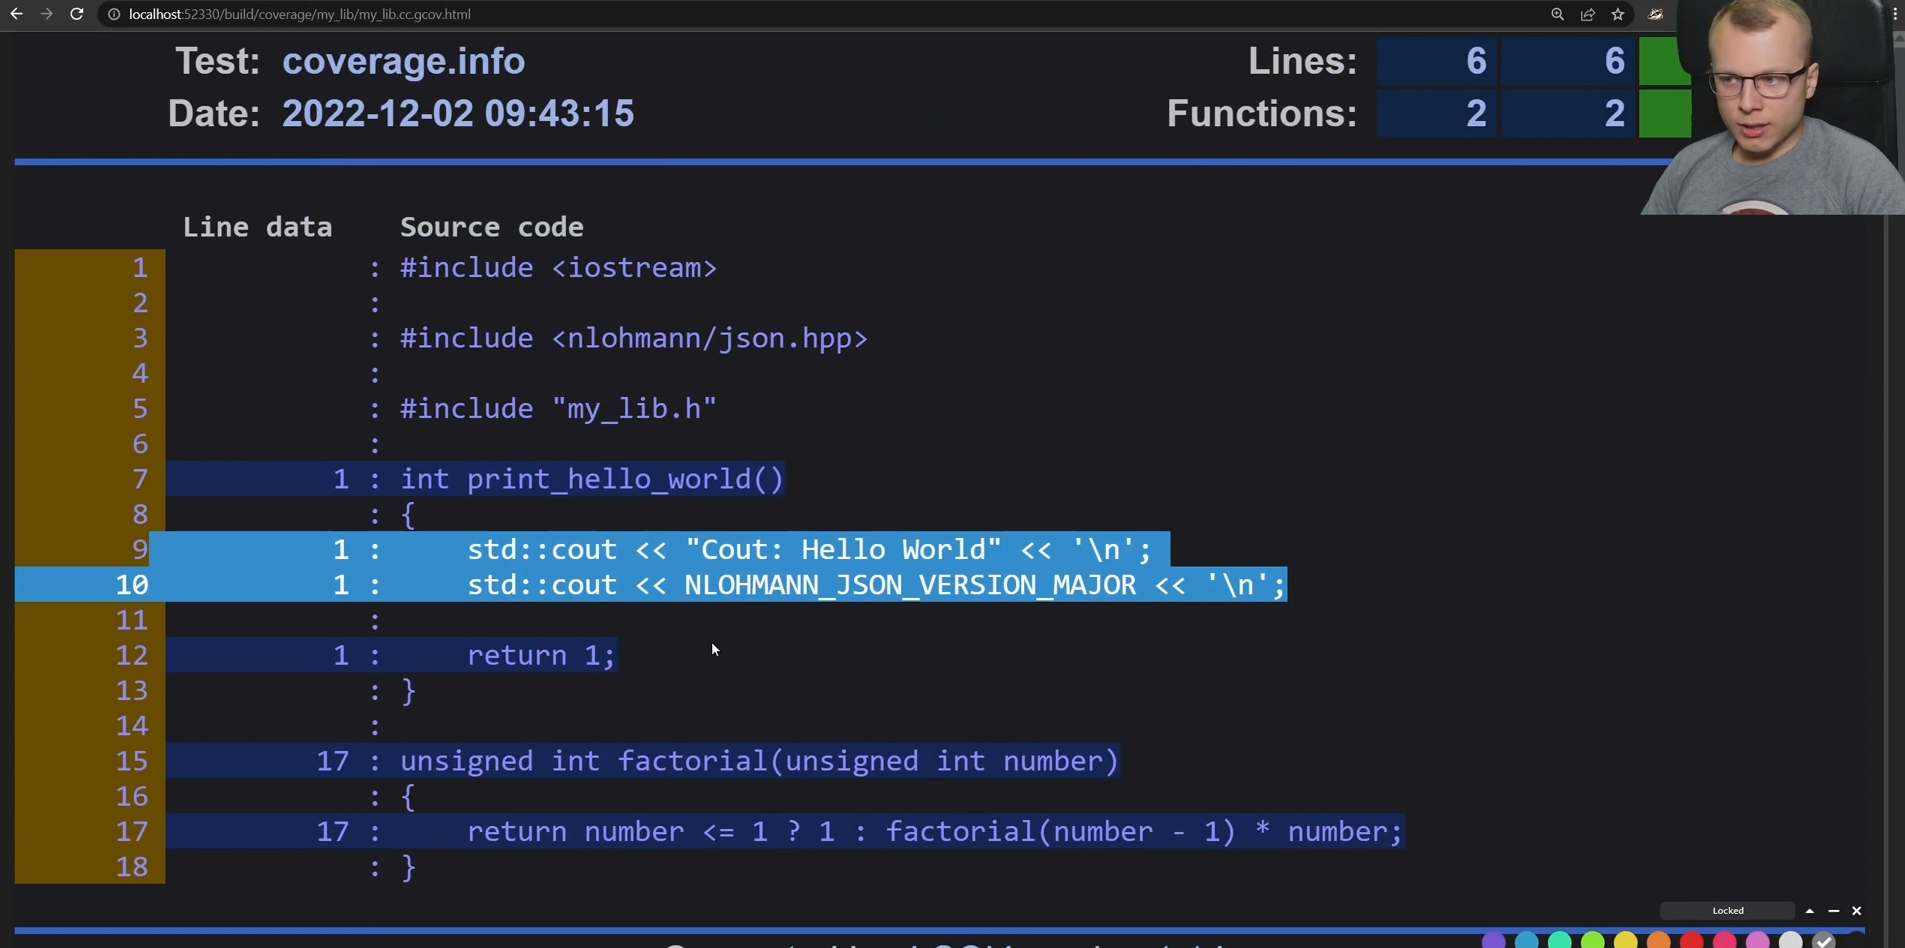
\includegraphics[width=5in]{cov2.png}
\end{center}



\subsection{Code Coverage.cmake}

\begin{verbatim}
include(CMakeParseArguments)

if(ENABLE_COVERAGE)
    # Check prereqs
    find_program(GCOV_PATH gcov)
    find_program(
        LCOV_PATH
        NAMES lcov
              lcov.bat
              lcov.exe
              lcov.perl)
    find_program(GENHTML_PATH NAMES genhtml genhtml.perl genhtml.bat)
    find_program(GCOVR_PATH gcovr PATHS ${CMAKE_SOURCE_DIR}/scripts/test)
    find_program(CPPFILT_PATH NAMES c++filt)

    if(NOT GCOV_PATH)
        message(FATAL_ERROR "gcov not found! Aborting...")
    endif() # NOT GCOV_PATH

    if(CMAKE_C_COMPILER_ID MATCHES "Clang" OR CMAKE_CXX_COMPILER_ID MATCHES
                                              "Clang")
        set(IS_CLANG TRUE)
    else()
        set(IS_CLANG FALSE)
    endif()
    if(CMAKE_C_COMPILER_ID MATCHES "GNU" OR CMAKE_CXX_COMPILER_ID MATCHES "GNU")
        set(IS_GCC TRUE)
    else()
        set(IS_GCC FALSE)
    endif()

    if(NOT ${IS_CLANG} AND NOT ${IS_GCC})
        message(FATAL_ERROR "Compiler is not gcc/clang! Aborting...")
    endif()

    set(COVERAGE_COMPILER_FLAGS "-g -O0 -fprofile-arcs -ftest-coverage")
    set(CMAKE_CXX_FLAGS_COVERAGE ${COVERAGE_COMPILER_FLAGS} FORCE)
    set(CMAKE_C_FLAGS_COVERAGE ${COVERAGE_COMPILER_FLAGS} FORCE)
    set(CMAKE_EXE_LINKER_FLAGS_COVERAGE "-lgcov" FORCE)
    set(CMAKE_SHARED_LINKER_FLAGS_COVERAGE "" FORCE)
    mark_as_advanced(
        CMAKE_CXX_FLAGS_COVERAGE
        CMAKE_C_FLAGS_COVERAGE
        CMAKE_EXE_LINKER_FLAGS_COVERAGE
        CMAKE_SHARED_LINKER_FLAGS_COVERAGE)

    if(NOT
       CMAKE_BUILD_TYPE
       STREQUAL
       "Debug")
        message(WARNING "Cov results with non-Debug build may be misleading")
    endif()

    if(${IS_GCC})
        link_libraries(gcov)
    endif()
endif()

# Defines a target for running and collection code coverage information Builds
# dependencies, runs the given executable and outputs reports. NOTE! The
# executable should always have a ZERO as exit code otherwise the coverage
# generation will not complete.
#
function(setup_target_for_coverage_lcov)
    set(options NO_DEMANGLE)
    set(oneValueArgs BASE_DIRECTORY NAME)
    set(multiValueArgs
        EXCLUDE
        EXECUTABLE
        EXECUTABLE_ARGS
        DEPENDENCIES
        LCOV_ARGS
        GENHTML_ARGS)
    cmake_parse_arguments(
        Coverage
        "${options}"
        "${oneValueArgs}"
        "${multiValueArgs}"
        ${ARGN})

    if(NOT LCOV_PATH)
        message(FATAL_ERROR "lcov not found! Aborting...")
    endif()
    if(NOT GENHTML_PATH)
        message(FATAL_ERROR "genhtml not found! Aborting...")
    endif()

    # Set base directory (as absolute path), or default to PROJECT_SOURCE_DIR
    if(${Coverage_BASE_DIRECTORY})
        get_filename_component(BASEDIR ${Coverage_BASE_DIRECTORY} ABSOLUTE)
    else()
        set(BASEDIR ${PROJECT_SOURCE_DIR})
    endif()

    # Collect excludes (CMake 3.4+: Also compute absolute paths)
    set(LCOV_EXCLUDES "")
    foreach(EXCLUDE ${Coverage_EXCLUDE} ${COVERAGE_EXCLUDES}
                    ${COVERAGE_LCOV_EXCLUDES})
        if(CMAKE_VERSION VERSION_GREATER 3.4)
            get_filename_component(
                EXCLUDE
                ${EXCLUDE}
                ABSOLUTE
                BASE_DIR
                ${BASEDIR})
        endif()
        list(APPEND LCOV_EXCLUDES "${EXCLUDE}")
    endforeach()
    list(REMOVE_DUPLICATES LCOV_EXCLUDES)

    # Conditional arguments
    if(CPPFILT_PATH AND NOT ${Coverage_NO_DEMANGLE})
        set(GENHTML_EXTRA_ARGS "--demangle-cpp")
    endif()

    # Setup target
    add_custom_target(
        ${Coverage_NAME}
        # Cleanup lcov
        COMMAND ${LCOV_PATH} ${Coverage_LCOV_ARGS} --gcov-tool ${GCOV_PATH}
                -directory . -b ${BASEDIR} --zerocounters
        # Create baseline to make sure untouched files show up in the report
        COMMAND ${LCOV_PATH} ${Coverage_LCOV_ARGS} --gcov-tool ${GCOV_PATH} -c
                -i -d . -b ${BASEDIR} -o ${Coverage_NAME}.base
        # Run tests
        COMMAND ${Coverage_EXECUTABLE} ${Coverage_EXECUTABLE_ARGS}
        # Capturing lcov counters and generating report
        COMMAND
            ${LCOV_PATH} ${Coverage_LCOV_ARGS} --gcov-tool ${GCOV_PATH}
            --directory . -b ${BASEDIR} --capture --output-file
            ${Coverage_NAME}.capture
        # add baseline counters
        COMMAND
            ${LCOV_PATH} ${Coverage_LCOV_ARGS} --gcov-tool ${GCOV_PATH} -a
            ${Coverage_NAME}.base -a ${Coverage_NAME}.capture --output-file
            ${Coverage_NAME}.total
        # filter collected data to final coverage report
        COMMAND
            ${LCOV_PATH} ${Coverage_LCOV_ARGS} --gcov-tool ${GCOV_PATH} --remove
            ${Coverage_NAME}.total ${LCOV_EXCLUDES} --output-file
            ${Coverage_NAME}.info
        # Generate HTML output
        COMMAND ${GENHTML_PATH} ${GENHTML_EXTRA_ARGS} ${Coverage_GENHTML_ARGS}
                -o ${Coverage_NAME} ${Coverage_NAME}.info
        # Set output files as GENERATED (will be removed on 'make clean')
        BYPRODUCTS ${Coverage_NAME}.base
                   ${Coverage_NAME}.capture
                   ${Coverage_NAME}.total
                   ${Coverage_NAME}.info
                   ${Coverage_NAME} # report directory
        WORKING_DIRECTORY ${PROJECT_BINARY_DIR}
        DEPENDS ${Coverage_DEPENDENCIES}
        VERBATIM # Protect arguments to commands
    )

    # Show where to find the lcov info report
    add_custom_command(
        TARGET ${Coverage_NAME}
        POST_BUILD
        COMMAND ;)

    # Show info where to find the report
    add_custom_command(
        TARGET ${Coverage_NAME}
        POST_BUILD
        COMMAND ;)
endfunction()

function(append_coverage_compiler_flags)
    set(CMAKE_C_FLAGS
        "${CMAKE_C_FLAGS} ${COVERAGE_COMPILER_FLAGS}"
        PARENT_SCOPE)
    set(CMAKE_CXX_FLAGS
        "${CMAKE_CXX_FLAGS} ${COVERAGE_COMPILER_FLAGS}"
        PARENT_SCOPE)
    message(
        STATUS
            "Appending code coverage compiler flags: ${COVERAGE_COMPILER_FLAGS}"
    )
endfunction()
\end{verbatim}


\section{Github Actions Continuous Integration}

Yml files instruct github to perform some actions when you push to the main branch. 
You can have unit testing automatically when you push for example.


\begin{center}
    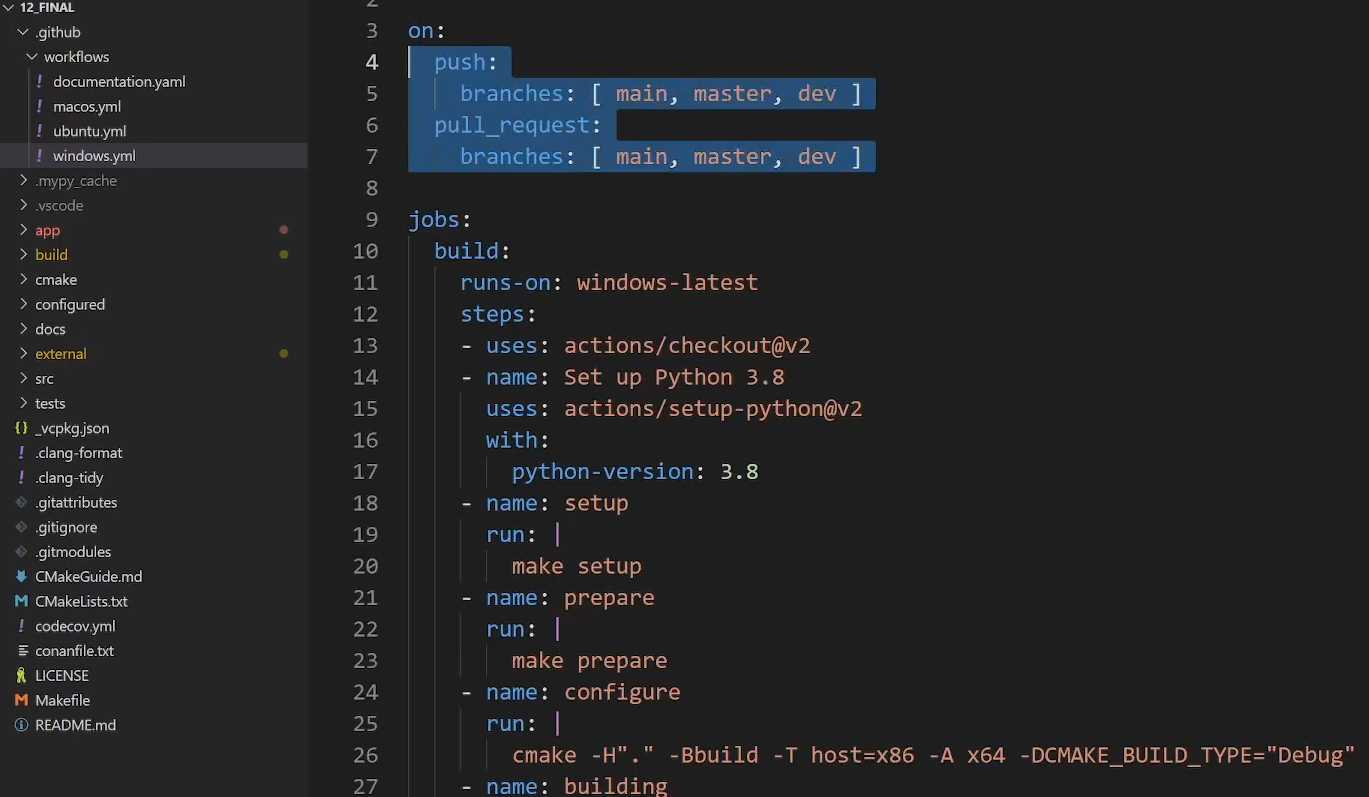
\includegraphics[width=4in]{actions.png}
\end{center}

For Ubuntu, you can have automatic code coverage as well. Not possible on macOS and Windows.


\subsection{Github Actions Workflows}

Follow your workflows, your different configurated unit tests on Github.


\begin{center}
    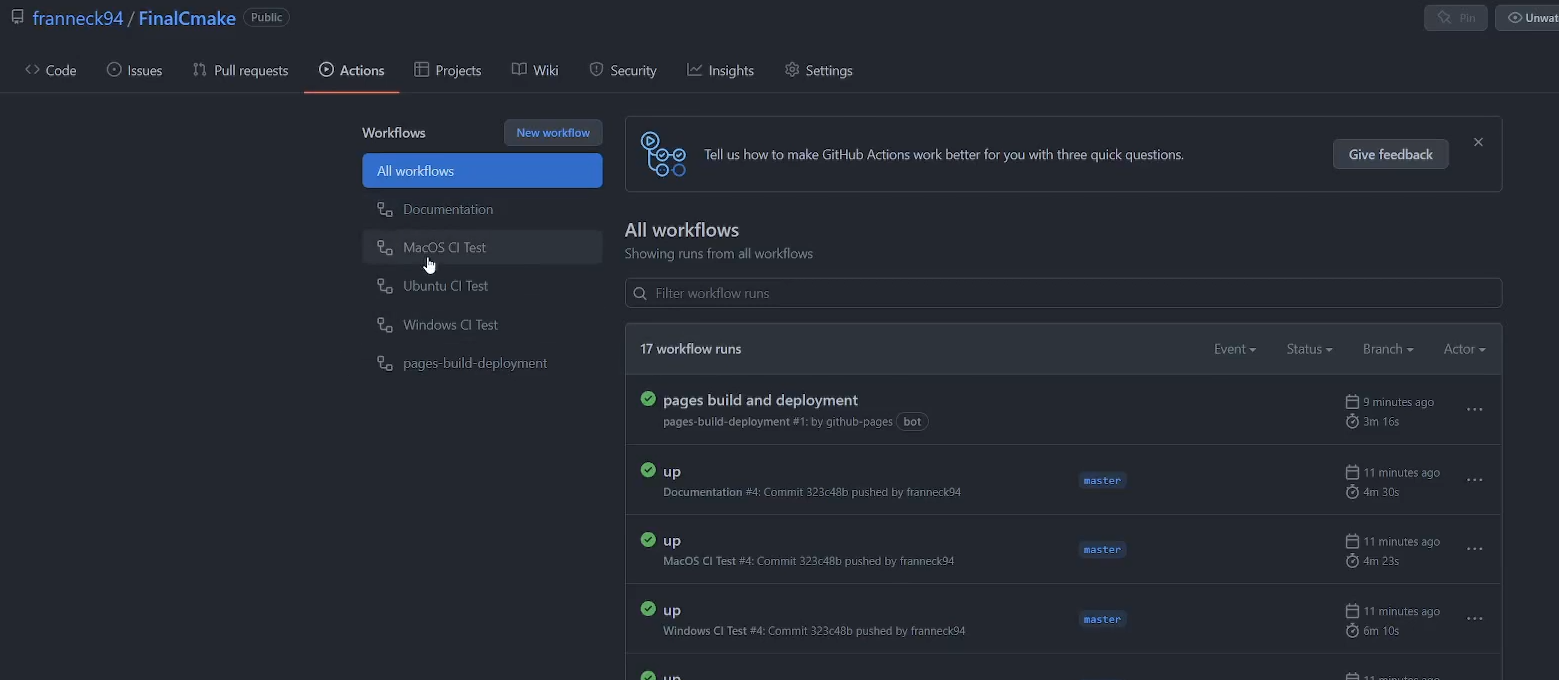
\includegraphics[width=2in]{actions2.png}
\end{center}

For every job configured, every step is executed on github, with a checkmark if everything has passed.


\begin{center}
    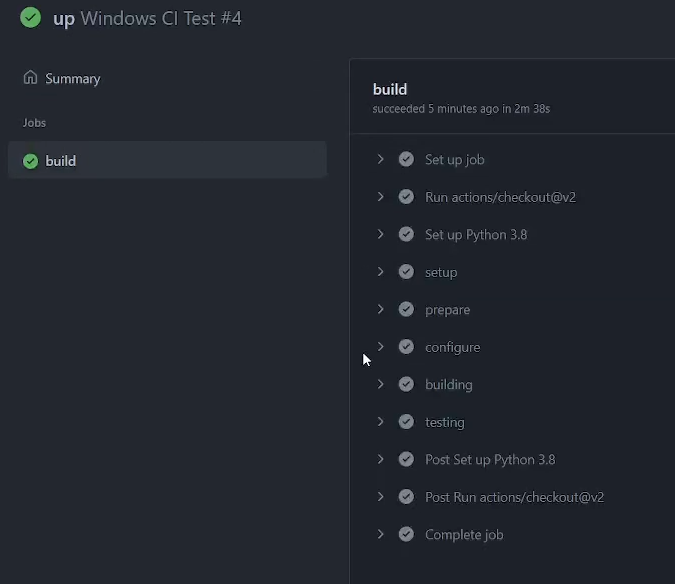
\includegraphics[width=2in]{actions3.png}
\end{center}

You can have great icons to see versions of the project passing on your github page.


\begin{center}
    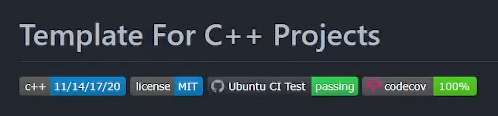
\includegraphics[width=2in]{actions4.png}
\end{center}


\begin{center}
    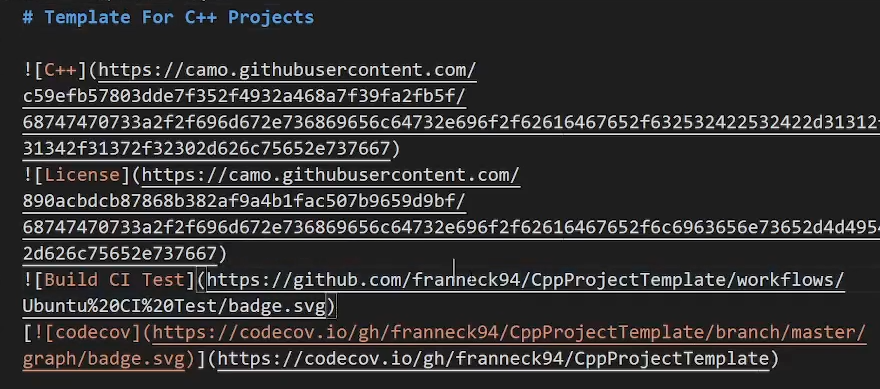
\includegraphics[width=2in]{actions5.png}
\end{center}


\subsection{Github Actions Codecov}

In Ubuntu, it is possible to upload the code coverage online, for free, automatically with github actions.

\begin{center}
    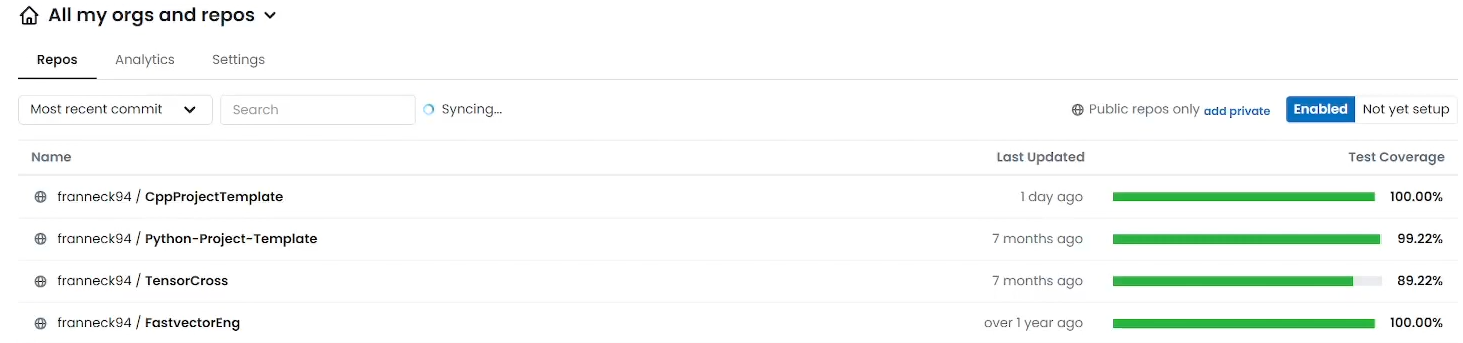
\includegraphics[width=5in]{codecov.png}
\end{center}

It is based on the Ubuntu.yaml configuration file.

\begin{center}
    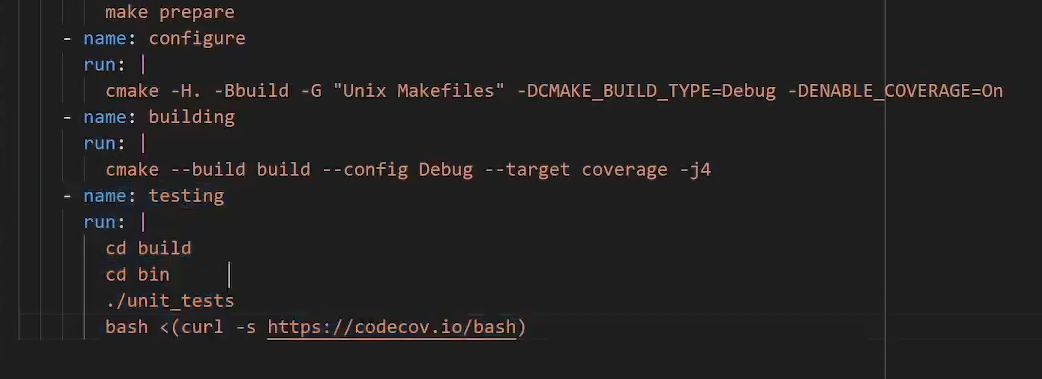
\includegraphics[width=5in]{codecov2.png}
\end{center}



\section{Pre-Commit}

When you have a github repo with your cpp project, you have many config files. Technically,
a user doesn't have to use any of your tools. However, there is a way to force him to do so, with 
Pre-Commit.


\subsection{Pre-Commit Installation}

Install pre-commit, a python program, with pip.

\begin{verbatim}
pip install pre-commit
\end{verbatim}


\subsection{Pre-Commit Configuration}

In your root directory, create a .pre-commit-config.yaml file.

\begin{verbatim}
fail_fast: false
repos:
-   repo: https://github.com/pre-commit/pre-commit-hooks
    rev: v4.4.0
    hooks:
      - id: check-yaml
      - id: check-json
        exclude: .vscode
      - id: end-of-file-fixer
      - id: trailing-whitespace

-   repo: https://github.com/pre-commit/mirrors-clang-format
    rev: 'v16.0.3'
    hooks:
      - id: clang-format
        exclude_types: [javascript, json]
\end{verbatim}

Then, run \$pre-commit install and \$pre-commit install-hooks commands from the project root.


\subsection{Pre-Commit in GitHub Actions Workflow Directory}

You can run Pre-Commit everytime there is a push on github branches with a pre-commit.yaml in the .github/workflow 
directory. It will run pre-commit on all pull requests as well!

\begin{verbatim}
name: pre-commit

on:
    pull_request:
    push:
        branches: [ main, master ]

jobs:
    pre-commit:
        runs-on: ubuntu-latest
        steps:
        - uses: actions/checkout@v2
        - uses: actions/setup python@v2
        - uses: pre-commit/action@2.0.0
\end{verbatim}


\section{Install Command for your Program}

We can make our build executable usable on your computer, just like any other tool. To make a transition from 
our project to our real computer, we will use an install command.


\subsection{Install in root CMakeLists.txt}

On linux, cmake install automatically on usr/local. On windows, it is in Programs directory.

\begin{verbatim}
install(TARGETS ${HE}
    EXPORT ${LIBA}
    ARCHIVE DESTINATION lib
    LIBRARY DESTINATION lib
    RUNTIME DESTINATION bin) 

install(TARGETS ${LIBA}
        ARCHIVE DESTINATION lib
        LIBRARY DESTINATION lib)

# in build

$ sudo cmake --build . --target install
\end{verbatim}


\begin{center}
    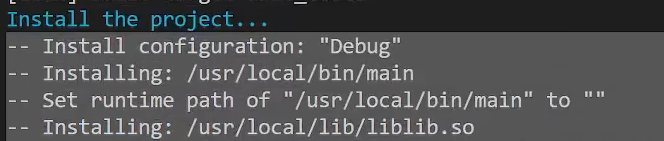
\includegraphics[width=2in]{inst.png}
\end{center}


\section{Jason Turner's Template}

\begin{verbatim}
lefticus/cmake_template // Jason Turner 2023 cmake starter pack

rename "myproject" in the cmake files to use it.

\end{verbatim}

\subsection{Jason Turner Tools Defaults- ProjectOptions.cmake}

\begin{verbatim}
Address sanitizer
Undefined behavior sanitizer
Fuzzing example built
Procedural optimization IPO (link time optimization)
Warnings as errors
Clang-tidy enabled
CPPcheck enabled
Options for precompiled headers
\end{verbatim}

\subsection{Hardening - Hardening.cmake}

\begin{verbatim}
Hardened compilation // make code safer
More compilation options / securities.

-fstack-protector
-fcf-protection
-fsanitize=undefined // undefined behavior sanitizer
-fno-sanitize-recover=undefined
-fsanitizise-minimal-runtime

+ debug information 
\end{verbatim}


\section{CMake Vim Plugins Combos}

\begin{verbatim}
See codevion/cpp2.md
\end{verbatim}

\section{COC - for code completion in nvim}
\begin{verbatim}
https://github.com/neoclide/coc.nvim
Jason Turner has this too
\end{verbatim}

\subsection{Pragma Once}

\begin{verbatim}
#pragma once is a non-standard directive that serves as an include guard. 
It ensures that a header file is included only once during the compilation process,
regardless of how many times it is referenced.

Placed at the beginning of a header file, it acts as a compiler directive to prevent multiple inclusions
Supported by most compilers, including GCC, Clang, and MSVC.
\end{verbatim}

\subsection{Glob - Include Many files with CMake}
 
You have at least two options. First, include every files one-by-one in the CMakeList.txt.
\begin{verbatim}
cmake_minimum_required(VERSION 3.10)
set(CMAKE_CXX_STANDARD 17)
set(CMAKE_CXX_STANDARD_REQUIRED ON)

project(hello VERSION 1.0) // traditional way to include files
add_executable(hello main.cpp Blah.cpp) // added here
target_include_directories(hello PUBLIC ${CMAKE_CURRENT_SOURCE_DIR}/include)
\end{verbatim}

Cmake discourages this glob method, but it is a more sane options for large projects.

\begin{verbatim}
file(GLOB_RECURSE SRC_FILES src/*.cpp) // glob everything in src/
add_executable(hello ${SRC_FILES})
\end{verbatim}

\textbf{In CMake - Traditionally Added}
\begin{verbatim}
add_executable(hello main.cpp src/Blah.cpp) // added here
\end{verbatim}

\textbf{In CMake - Globing}
\begin{verbatim}
file(GLOB_RECURSE SRC_FILES src/*.cpp)
add_executable(hello main.cpp ${SRC_FILES})
\end{verbatim}

\section{Jason Turner's CMake Template - Options}

\begin{verbatim}
include(cmake/SystemLink.cmake)
include(cmake/LibFuzzer.cmake)
include(CMakeDependentOption)
include(CheckCXXCompilerFlag)

macro(myproject_supports_sanitizers)
  if((CMAKE_CXX_COMPILER_ID MATCHES ".*Clang.*" OR CMAKE_CXX_COMPILER_ID MATCHES ".*GNU.*") AND NOT WIN32)
    set(SUPPORTS_UBSAN ON)
  else()
    set(SUPPORTS_UBSAN OFF)
  endif()

  if((CMAKE_CXX_COMPILER_ID MATCHES ".*Clang.*" OR CMAKE_CXX_COMPILER_ID MATCHES ".*GNU.*") AND WIN32)
    set(SUPPORTS_ASAN OFF)
  else()
    set(SUPPORTS_ASAN ON)
  endif()
endmacro()

macro(myproject_setup_options)
  option(myproject_ENABLE_HARDENING "Enable hardening" ON)
  option(myproject_ENABLE_COVERAGE "Enable coverage reporting" OFF)
  cmake_dependent_option(
    myproject_ENABLE_GLOBAL_HARDENING
    "Attempt to push hardening options to built dependencies"
    ON
    myproject_ENABLE_HARDENING
    OFF)

  myproject_supports_sanitizers()

  if(NOT PROJECT_IS_TOP_LEVEL OR myproject_PACKAGING_MAINTAINER_MODE)
    option(myproject_ENABLE_IPO "Enable IPO/LTO" OFF)
    option(myproject_WARNINGS_AS_ERRORS "Treat Warnings As Errors" OFF)
    option(myproject_ENABLE_USER_LINKER "Enable user-selected linker" OFF)
    option(myproject_ENABLE_SANITIZER_ADDRESS "Enable address sanitizer" OFF)
    option(myproject_ENABLE_SANITIZER_LEAK "Enable leak sanitizer" OFF)
    option(myproject_ENABLE_SANITIZER_UNDEFINED "Enable undefined sanitizer" OFF)
    option(myproject_ENABLE_SANITIZER_THREAD "Enable thread sanitizer" OFF)
    option(myproject_ENABLE_SANITIZER_MEMORY "Enable memory sanitizer" OFF)
    option(myproject_ENABLE_UNITY_BUILD "Enable unity builds" OFF)
    option(myproject_ENABLE_CLANG_TIDY "Enable clang-tidy" OFF)
    option(myproject_ENABLE_CPPCHECK "Enable cpp-check analysis" OFF)
    option(myproject_ENABLE_PCH "Enable precompiled headers" OFF)
    option(myproject_ENABLE_CACHE "Enable ccache" OFF)
  else()
    option(myproject_ENABLE_IPO "Enable IPO/LTO" ON)
    option(myproject_WARNINGS_AS_ERRORS "Treat Warnings As Errors" ON)
    option(myproject_ENABLE_USER_LINKER "Enable user-selected linker" OFF)
    option(myproject_ENABLE_SANITIZER_ADDRESS "Enable address sanitizer" ${SUPPORTS_ASAN})
    option(myproject_ENABLE_SANITIZER_LEAK "Enable leak sanitizer" OFF)
    option(myproject_ENABLE_SANITIZER_UNDEFINED "Enable undefined sanitizer" ${SUPPORTS_UBSAN})
    option(myproject_ENABLE_SANITIZER_THREAD "Enable thread sanitizer" OFF)
    option(myproject_ENABLE_SANITIZER_MEMORY "Enable memory sanitizer" OFF)
    option(myproject_ENABLE_UNITY_BUILD "Enable unity builds" OFF)
    option(myproject_ENABLE_CLANG_TIDY "Enable clang-tidy" ON)
    option(myproject_ENABLE_CPPCHECK "Enable cpp-check analysis" ON)
    option(myproject_ENABLE_PCH "Enable precompiled headers" OFF)
    option(myproject_ENABLE_CACHE "Enable ccache" ON)
  endif()

  if(NOT PROJECT_IS_TOP_LEVEL)
    mark_as_advanced(
      myproject_ENABLE_IPO
      myproject_WARNINGS_AS_ERRORS
      myproject_ENABLE_USER_LINKER
      myproject_ENABLE_SANITIZER_ADDRESS
      myproject_ENABLE_SANITIZER_LEAK
      myproject_ENABLE_SANITIZER_UNDEFINED
      myproject_ENABLE_SANITIZER_THREAD
      myproject_ENABLE_SANITIZER_MEMORY
      myproject_ENABLE_UNITY_BUILD
      myproject_ENABLE_CLANG_TIDY
      myproject_ENABLE_CPPCHECK
      myproject_ENABLE_COVERAGE
      myproject_ENABLE_PCH
      myproject_ENABLE_CACHE)
  endif()

  myproject_check_libfuzzer_support(LIBFUZZER_SUPPORTED)
  if(LIBFUZZER_SUPPORTED AND (myproject_ENABLE_SANITIZER_ADDRESS OR myproject_ENABLE_SANITIZER_THREAD OR myproject_ENABLE_SANITIZER_UNDEFINED))
    set(DEFAULT_FUZZER ON)
  else()
    set(DEFAULT_FUZZER OFF)
  endif()

  option(myproject_BUILD_FUZZ_TESTS "Enable fuzz testing executable" ${DEFAULT_FUZZER})

endmacro()

macro(myproject_global_options)
  if(myproject_ENABLE_IPO)
    include(cmake/InterproceduralOptimization.cmake)
    myproject_enable_ipo()
  endif()

  myproject_supports_sanitizers()

  if(myproject_ENABLE_HARDENING AND myproject_ENABLE_GLOBAL_HARDENING)
    include(cmake/Hardening.cmake)
    if(NOT SUPPORTS_UBSAN 
       OR myproject_ENABLE_SANITIZER_UNDEFINED
       OR myproject_ENABLE_SANITIZER_ADDRESS
       OR myproject_ENABLE_SANITIZER_THREAD
       OR myproject_ENABLE_SANITIZER_LEAK)
      set(ENABLE_UBSAN_MINIMAL_RUNTIME FALSE)
    else()
      set(ENABLE_UBSAN_MINIMAL_RUNTIME TRUE)
    endif()
    message("${myproject_ENABLE_HARDENING} ${ENABLE_UBSAN_MINIMAL_RUNTIME} ${myproject_ENABLE_SANITIZER_UNDEFINED}")
    myproject_enable_hardening(myproject_options ON ${ENABLE_UBSAN_MINIMAL_RUNTIME})
  endif()
endmacro()

macro(myproject_local_options)
  if(PROJECT_IS_TOP_LEVEL)
    include(cmake/StandardProjectSettings.cmake)
  endif()

  add_library(myproject_warnings INTERFACE)
  add_library(myproject_options INTERFACE)

  include(cmake/CompilerWarnings.cmake)
  myproject_set_project_warnings(
    myproject_warnings
    ${myproject_WARNINGS_AS_ERRORS}
    ""
    ""
    ""
    "")

  if(myproject_ENABLE_USER_LINKER)
    include(cmake/Linker.cmake)
    configure_linker(myproject_options)
  endif()

  include(cmake/Sanitizers.cmake)
  myproject_enable_sanitizers(
    myproject_options
    ${myproject_ENABLE_SANITIZER_ADDRESS}
    ${myproject_ENABLE_SANITIZER_LEAK}
    ${myproject_ENABLE_SANITIZER_UNDEFINED}
    ${myproject_ENABLE_SANITIZER_THREAD}
    ${myproject_ENABLE_SANITIZER_MEMORY})

  set_target_properties(myproject_options PROPERTIES UNITY_BUILD ${myproject_ENABLE_UNITY_BUILD})

  if(myproject_ENABLE_PCH)
    target_precompile_headers(
      myproject_options
      INTERFACE
      <vector>
      <string>
      <utility>)
  endif()

  if(myproject_ENABLE_CACHE)
    include(cmake/Cache.cmake)
    myproject_enable_cache()
  endif()

  include(cmake/StaticAnalyzers.cmake)
  if(myproject_ENABLE_CLANG_TIDY)
    myproject_enable_clang_tidy(myproject_options ${myproject_WARNINGS_AS_ERRORS})
  endif()

  if(myproject_ENABLE_CPPCHECK)
    myproject_enable_cppcheck(${myproject_WARNINGS_AS_ERRORS} "" # override cppcheck options
    )
  endif()

  if(myproject_ENABLE_COVERAGE)
    include(cmake/Tests.cmake)
    myproject_enable_coverage(myproject_options)
  endif()

  if(myproject_WARNINGS_AS_ERRORS)
    check_cxx_compiler_flag("-Wl,--fatal-warnings" LINKER_FATAL_WARNINGS)
    if(LINKER_FATAL_WARNINGS)
      # This is not working consistently, so disabling for now
      # target_link_options(myproject_options INTERFACE -Wl,--fatal-warnings)
    endif()
  endif()

  if(myproject_ENABLE_HARDENING AND NOT myproject_ENABLE_GLOBAL_HARDENING)
    include(cmake/Hardening.cmake)
    if(NOT SUPPORTS_UBSAN 
       OR myproject_ENABLE_SANITIZER_UNDEFINED
       OR myproject_ENABLE_SANITIZER_ADDRESS
       OR myproject_ENABLE_SANITIZER_THREAD
       OR myproject_ENABLE_SANITIZER_LEAK)
      set(ENABLE_UBSAN_MINIMAL_RUNTIME FALSE)
    else()
      set(ENABLE_UBSAN_MINIMAL_RUNTIME TRUE)
    endif()
    myproject_enable_hardening(myproject_options OFF ${ENABLE_UBSAN_MINIMAL_RUNTIME})
  endif()

endmacro()
\end{verbatim}
